% Options for packages loaded elsewhere
\PassOptionsToPackage{unicode}{hyperref}
\PassOptionsToPackage{hyphens}{url}
\documentclass[
  ignorenonframetext,
  aspectratio=169,
]{beamer}
\newif\ifbibliography
\usepackage{pgfpages}
\setbeamertemplate{caption}[numbered]
\setbeamertemplate{caption label separator}{: }
\setbeamercolor{caption name}{fg=normal text.fg}
\beamertemplatenavigationsymbolsempty
% remove section numbering
\setbeamertemplate{part page}{
  \centering
  \begin{beamercolorbox}[sep=16pt,center]{part title}
    \usebeamerfont{part title}\insertpart\par
  \end{beamercolorbox}
}
\setbeamertemplate{section page}{
  \centering
  \begin{beamercolorbox}[sep=12pt,center]{section title}
    \usebeamerfont{section title}\insertsection\par
  \end{beamercolorbox}
}
\setbeamertemplate{subsection page}{
  \centering
  \begin{beamercolorbox}[sep=8pt,center]{subsection title}
    \usebeamerfont{subsection title}\insertsubsection\par
  \end{beamercolorbox}
}
% Prevent slide breaks in the middle of a paragraph
\widowpenalties 1 10000
\raggedbottom
\AtBeginPart{
  \frame{\partpage}
}
\AtBeginSection{
  \ifbibliography
  \else
    \frame{\sectionpage}
  \fi
}
\AtBeginSubsection{
  \frame{\subsectionpage}
}
\usepackage{iftex}
\ifPDFTeX
  \usepackage[T1]{fontenc}
  \usepackage[utf8]{inputenc}
  \usepackage{textcomp} % provide euro and other symbols
\else % if luatex or xetex
  \usepackage{unicode-math} % this also loads fontspec
  \defaultfontfeatures{Scale=MatchLowercase}
  \defaultfontfeatures[\rmfamily]{Ligatures=TeX,Scale=1}
\fi
\usepackage{lmodern}
\ifPDFTeX\else
  % xetex/luatex font selection
\fi
% Use upquote if available, for straight quotes in verbatim environments
\IfFileExists{upquote.sty}{\usepackage{upquote}}{}
\IfFileExists{microtype.sty}{% use microtype if available
  \usepackage[]{microtype}
  \UseMicrotypeSet[protrusion]{basicmath} % disable protrusion for tt fonts
}{}
\makeatletter
\@ifundefined{KOMAClassName}{% if non-KOMA class
  \IfFileExists{parskip.sty}{%
    \usepackage{parskip}
  }{% else
    \setlength{\parindent}{0pt}
    \setlength{\parskip}{6pt plus 2pt minus 1pt}}
}{% if KOMA class
  \KOMAoptions{parskip=half}}
\makeatother
\usepackage{longtable,booktabs,array}
\usepackage{caption}
\captionsetup[table]{skip=6pt}
\newcounter{none} % for unnumbered tables
\usepackage{calc} % for calculating minipage widths
\usepackage{caption}
% Make caption package work with longtable
\makeatletter
\def\fnum@table{\tablename~\thetable}
\makeatother
\usepackage{graphicx}
\makeatletter
\newsavebox\pandoc@box
\newcommand*\pandocbounded[1]{% scales image to fit in text height/width
  \sbox\pandoc@box{#1}%
  \Gscale@div\@tempa{\textheight}{\dimexpr\ht\pandoc@box+\dp\pandoc@box\relax}%
  \Gscale@div\@tempb{\linewidth}{\wd\pandoc@box}%
  \ifdim\@tempb\p@<\@tempa\p@\let\@tempa\@tempb\fi% select the smaller of both
  \ifdim\@tempa\p@<\p@\scalebox{\@tempa}{\usebox\pandoc@box}%
  \else\usebox{\pandoc@box}%
  \fi%
}
% Set default figure placement to htbp
\def\fps@figure{htbp}
\makeatother
\setlength{\emergencystretch}{3em} % prevent overfull lines
\providecommand{\tightlist}{%
  \setlength{\itemsep}{0pt}\setlength{\parskip}{0pt}}
% Auto-generated by infrastructure/rendering/_pdf_latex_helpers.py::extract_math_font_preamble.
% Minimal header passed to Pandoc via -H so Beamer slides pick up the same math font
% as the combined-PDF path. Adjust the manuscript's preamble.md to change the font globally.
\usepackage{unicode-math}
\setmathfont{latinmodern-math.otf}

% Manuscript macro/package fallbacks (newcommand -> providecommand).
% Core mathematics
\usepackage{amsmath}
\usepackage{amssymb}
% Document layout
% Tables
\usepackage{booktabs}
% Caption styling (booktabs already loaded above). Small caption font with a
% bold label ("Figure 1", "Table 2") gives the math/figure-heavy layout a
% consistent, journal-like caption rhythm without fighting pandoc-crossref —
% pandoc emits standard \caption{}, and caption/captionsetup only restyle it.
% ── Theorem environments ─────────────────────────────────────────────────
% amsthm is loaded above. The FedGVI<->Friston bridge is stated as a small
% number of theorems/definitions/lemmas/propositions/corollaries; sharing one
% counter (definition/lemma/proposition/corollary all step the `theorem`
% counter) gives a single monotone numbering 1, 2, 3, ... across all kinds, so
% authors can reference them as Theorem 1, Definition 2, Corollary 3 without a
% per-kind counter drifting out of order. Plain style for theorem-like results,
% definition style (upright body) for definitions.
% (algorithm2e intentionally not loaded: this manuscript states results as
% numbered amsthm Theorems/Definitions, not algorithm2e pseudocode.)
% Code listings
\usepackage{listings}
% Typography and formatting
% (siunitx intentionally not loaded: no \SI/\num units appear in this manuscript.)
% Cross-references and citations
% (cleveref and titlesec intentionally not loaded: unavailable in this TeX tree
% and not required. Cross-references resolve through pandoc-crossref's own
% \ref-style names — no \cref appears — and section heading styling falls back
% to the pandoc/LaTeX defaults.)
% ── TeX Live Basic-compatible mono font for code listings ────────────
% Latin Modern Mono is bundled with TeX Live Basic and keeps the manuscript
% renderable on minimal TeX installations. Mathematical Unicode coverage is
% provided separately by Latin Modern Math below, so the code font does not
% need a private JuliaMono installation.
%
% Use the TeX font filename rather than the system-family name: the minimal
% TeX Live fontconfig database may not register the OpenType family even though
% kpsewhich can resolve the bundled files.
% Math font for unicode-math: Latin Modern Math (TeX Live) has full BMP
% coverage including U+2223 (\mid), U+226A/226B (\ll/\gg), and the Greek/
% blackboard letters used in equations. Without an explicit \setmathfont,
% unicode-math falls back to lmroman text font which lacks several glyphs
% and emits "Missing character" warnings on every \mid in math mode.

% Slide layout defaults for warning-clean scientific decks.
\usepackage{etoolbox}
\IfFileExists{xurl.sty}{\usepackage{xurl}}{}
\IfFileExists{seqsplit.sty}{\usepackage{seqsplit}}{\newcommand{\seqsplit}[1]{#1}}
\protected\def\breakseq#1{\seqsplit{#1}}
\protected\def\breaktt#1{\begingroup\ttfamily\seqsplit{#1}\endgroup}
\setlength{\emergencystretch}{6em}
\tolerance=5000
\hbadness=10000
\hfuzz=1pt
\setlength{\tabcolsep}{2pt}
\AtBeginEnvironment{longtable}{\tiny\renewcommand{\arraystretch}{0.86}\setlength{\tabcolsep}{1pt}}
\AtBeginEnvironment{tabular}{\tiny\renewcommand{\arraystretch}{0.86}\setlength{\tabcolsep}{1pt}}
\AtBeginEnvironment{equation}{\tiny}
\AtBeginEnvironment{equation*}{\tiny}
\AtBeginEnvironment{align}{\tiny}
\AtBeginEnvironment{align*}{\tiny}
\AtBeginEnvironment{itemize}{\footnotesize}
\AtBeginEnvironment{enumerate}{\footnotesize}
\AtBeginEnvironment{description}{\footnotesize}
\setbeamerfont{caption}{size=\tiny}
\setbeamerfont{caption name}{size=\tiny}
\setbeamerfont{normal text}{size=\small}
\setbeamerfont{frametitle}{size=\small}
\setbeamerfont{section title}{size=\footnotesize}
\setbeamerfont{subsection title}{size=\footnotesize}
\setbeamertemplate{section page}{%
  \centering
  \begin{beamercolorbox}[sep=12pt,center,wd=\paperwidth]{section title}
    \parbox{0.86\paperwidth}{\centering\usebeamerfont{section title}\insertsection\par}
  \end{beamercolorbox}
}
\setbeamertemplate{subsection page}{%
  \centering
  \begin{beamercolorbox}[sep=8pt,center,wd=\paperwidth]{subsection title}
    \parbox{0.86\paperwidth}{\centering\usebeamerfont{subsection title}\insertsubsection\par}
  \end{beamercolorbox}
}
\setlength{\abovecaptionskip}{2pt}
\setlength{\belowcaptionskip}{0pt}

% Natbib and cross-reference fallbacks — slides don't load natbib
% or cleveref, but combined-PDF manuscript prose may emit these
% commands. The fallback renders citations as a bracketed key list
% and cross-references as detokenized labels so slides don't fail on
% undefined control sequences or raw underscores. \providecommand is
% a no-op if packages load later.
\providecommand{\citep}[1]{[#1]}
\providecommand{\citet}[1]{#1}
\providecommand{\citealp}[1]{#1}
\providecommand{\citeauthor}[1]{#1}
\providecommand{\citeyear}[1]{#1}
\providecommand{\cref}[1]{\texttt{\detokenize{#1}}}
\providecommand{\Cref}[1]{\texttt{\detokenize{#1}}}
\providecommand{\crefrange}[2]{\texttt{\detokenize{#1}}--\texttt{\detokenize{#2}}}
\providecommand{\Crefrange}[2]{\texttt{\detokenize{#1}}--\texttt{\detokenize{#2}}}
\providecommand{\paragraph}[1]{\textbf{#1}\ }

% Opt-in accessible presentation profile.
\setbeamerfont{normal text}{size*={20pt}{24pt}}
\setbeamerfont{frametitle}{size*={28pt}{32pt}}
\setbeamerfont{section title}{size*={28pt}{32pt}}
\setbeamerfont{subsection title}{size*={28pt}{32pt}}
\setbeamerfont{caption}{size*={16pt}{19pt}}
\setbeamerfont{caption name}{size*={16pt}{19pt}}
\setbeamerfont{itemize/enumerate body}{size*={20pt}{24pt}}
\setbeamerfont{itemize/enumerate subbody}{size*={20pt}{24pt}}
\setbeamerfont{itemize/enumerate subsubbody}{size*={20pt}{24pt}}
\setbeamerfont{itemize item}{size*={20pt}{24pt}}
\setbeamerfont{itemize subitem}{size*={20pt}{24pt}}
\setbeamerfont{itemize subsubitem}{size*={20pt}{24pt}}
\setbeamerfont{description body}{size*={20pt}{24pt}}
\setbeamerfont{description item}{size*={20pt}{24pt}}
\setbeamerfont{quote}{size*={20pt}{24pt}}
\setbeamerfont{quotation}{size*={20pt}{24pt}}
\AtBeginEnvironment{longtable}{\fontsize{20pt}{24pt}\selectfont}
\AtBeginEnvironment{tabular}{\fontsize{20pt}{24pt}\selectfont}
\AtBeginEnvironment{equation}{\fontsize{20pt}{24pt}\selectfont}
\AtBeginEnvironment{equation*}{\fontsize{20pt}{24pt}\selectfont}
\AtBeginEnvironment{align}{\fontsize{20pt}{24pt}\selectfont}
\AtBeginEnvironment{align*}{\fontsize{20pt}{24pt}\selectfont}
\AtBeginEnvironment{itemize}{\fontsize{20pt}{24pt}\selectfont}
\AtBeginEnvironment{enumerate}{\fontsize{20pt}{24pt}\selectfont}
\AtBeginEnvironment{description}{\fontsize{20pt}{24pt}\selectfont}
\AtBeginDocument{\usebeamerfont{normal text}}
\newlength{\AFSlideTableWidth}
% The fixed footer reservation is calibrated with the semantic seven-line regular-body budget.
\setbeamertemplate{footline}{%
  \leavevmode\vbox{%
    \hbox{%
      \begin{beamercolorbox}[wd=\paperwidth,ht=16pt,dp=3pt,center]{author in head/foot}%
        \fontsize{16pt}{19pt}\selectfont Untagged PDF derivative \textbar\ \href{../web/index.html}{HTML reader}%
      \end{beamercolorbox}%
    }%
    \vskip6pt%
  }%
}
% Accessible footer reserved height: 25pt.

\newtheorem{proposition}{Proposition}
\newtheorem{hypothesis}{Hypothesis}
\newtheorem{remark}[theorem]{Remark}
\newtheorem{axiom}{Axiom}
\newtheorem{property}{Property}
\usepackage{bookmark}
\IfFileExists{xurl.sty}{\usepackage{xurl}}{} % add URL line breaks if available
\urlstyle{same}
% fallback for those not using the hyperref driver hyperxmp:
\makeatletter
\@ifundefined{xmpquote}{\newcommand{\xmpquote}[1]{#1}}{}
\makeatother
\hypersetup{
  hidelinks,
  pdfcreator={LaTeX via pandoc}}

\author{\texorpdfstring{}{}}
\date{}

\begin{document}

\section{Abstract}\label{sec:abstract}

\begin{frame}{Abstract}
Multi-agent active inference gives a natural account of belief sharing:
agents hold local posteriors over a shared latent state, communicate
those beliefs, and pool them into a colony-level consensus. The same
mechanism is fragile when a member is miscalibrated, corrupted, or
strategically wrong.
\end{frame}

\begin{frame}{Abstract (part 2)}
Because the standard pool multiplies the reports together, a single
confident-but-wrong broadcast that puts near-zero mass on the true state
can pull the whole consensus off it, outweighing many honest members.
\end{frame}

\begin{frame}{Abstract (part 3)}
The colony therefore needs a way to preserve the useful structure of
belief sharing while limiting the influence of contaminated beliefs.
\end{frame}

\begin{frame}{Abstract (part 4)}
This paper presents Active Fedference, a discrete-categorical framework
that connects robust federated generalized variational inference with
active inference belief sharing. The main bridge is structural: standard
belief sharing appears as the non-robust corner of a broader
generalized-Bayes family,
\end{frame}

\begin{frame}{Abstract (part 5)}
while robust losses, conservative server fusion, and explicit
aggregation diagnostics describe how the system moves away from that
corner under declared contamination mechanisms.
\end{frame}

\begin{frame}{Abstract (part 6)}
The result is not a replacement for belief sharing, but a containment
result: ordinary belief sharing is recovered when robustness is turned
off. Bounded-loss theory applies on the client axis, while the
variational-server axis supplies an objective-backed redescending weight
update.
\end{frame}

\begin{frame}{Abstract (part 7)}
Following the manuscript's authoritative three-axis guarantee map, the
paper keeps source-conditional client updates, a recovery-only heuristic
server rule, and an objective-backed variational server rule as separate
claim owners, with no robustness guarantee transferred between them.
\end{frame}

\begin{frame}{Abstract (part 8)}
The study suite then exercises the framework as an end-to-end research
system: recovery checks anchor the standard-Bayes limit, belief-sharing
studies verify the communication baseline, contamination experiments
test robust consensus, and extension studies probe moving agents,
hierarchical latent structure,
\end{frame}

\begin{frame}{Abstract (part 9)}
sensitivity to acuity and colony size, parameter recovery, and
single-host socket-backed federation traces.
\end{frame}

\begin{frame}{Abstract (part 10)}
All reported quantities are generated from deterministic analysis
artifacts and injected into the manuscript by token, so the paper,
figures, release package, and validation reports remain tied to the same
execution record.
\end{frame}

\begin{frame}{Abstract (part 11)}
The open-source repository is
ActiveInferenceInstitute/Active\_Fedference. This final-release
manuscript uses assigned version DOI
\href{https://doi.org/10.5281/zenodo.22149133}{10.5281/zenodo.22149133};
the bound deposited PDF and repository release are controlled by
separate publication gates.
\end{frame}

\begin{frame}{Abstract (part 12)}
\textbf{Keywords:} active inference, federated learning, generalised
variational inference, belief sharing, robustness, FedGVI

The complete system schematic is shown in
fig.~1.
\end{frame}

\begin{frame}{Abstract (part 13)}
\begin{figure}
\centering
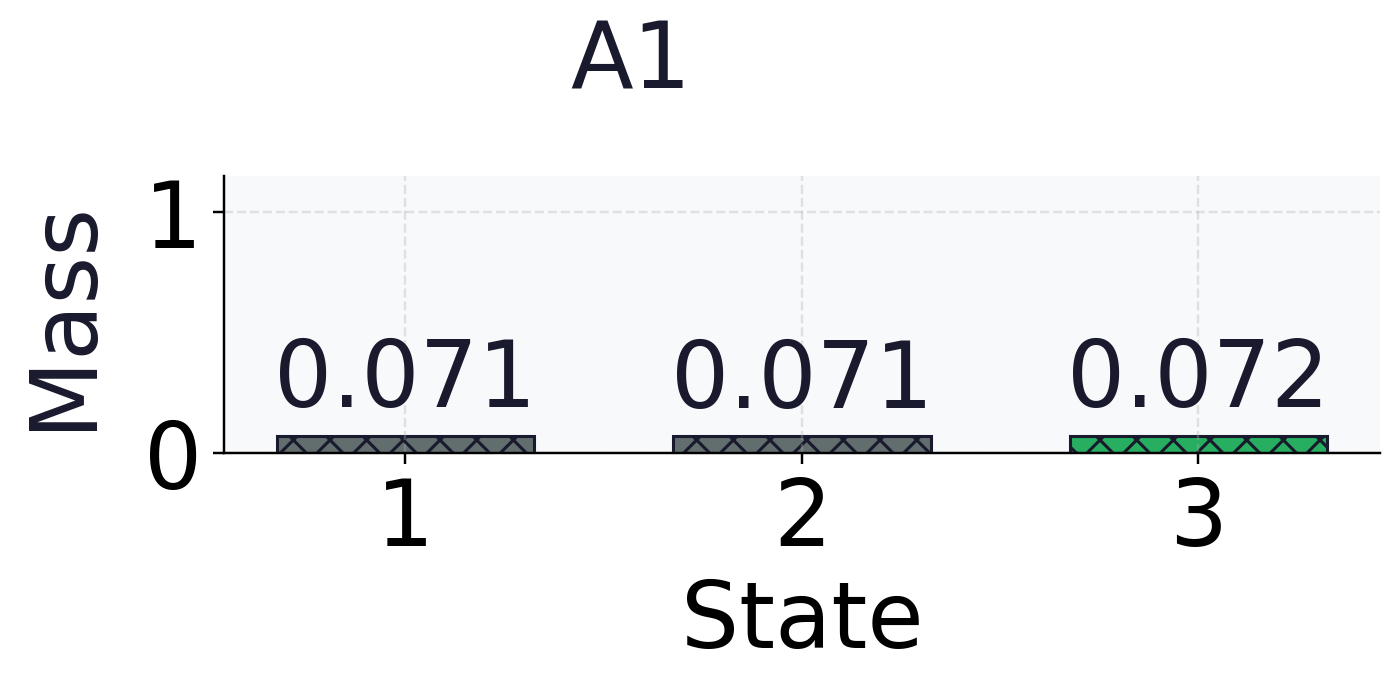
\includegraphics[keepaspectratio,width=0.98\linewidth,height=0.8\textheight,alt={A1: source-derived posterior masses for states 1 to 3, common 0--1 probability scale; arrow marks this row\textquotesingle s argmax when present.}]{../figures/graphical_abstract.slide-row-1-states-1-3.png}
\refstepcounter{figure}\label{fig:graphical-abstract-slide-panel-1}
\end{figure}
\end{frame}

\begin{frame}{Abstract (part 14)}
\begin{figure}
\centering
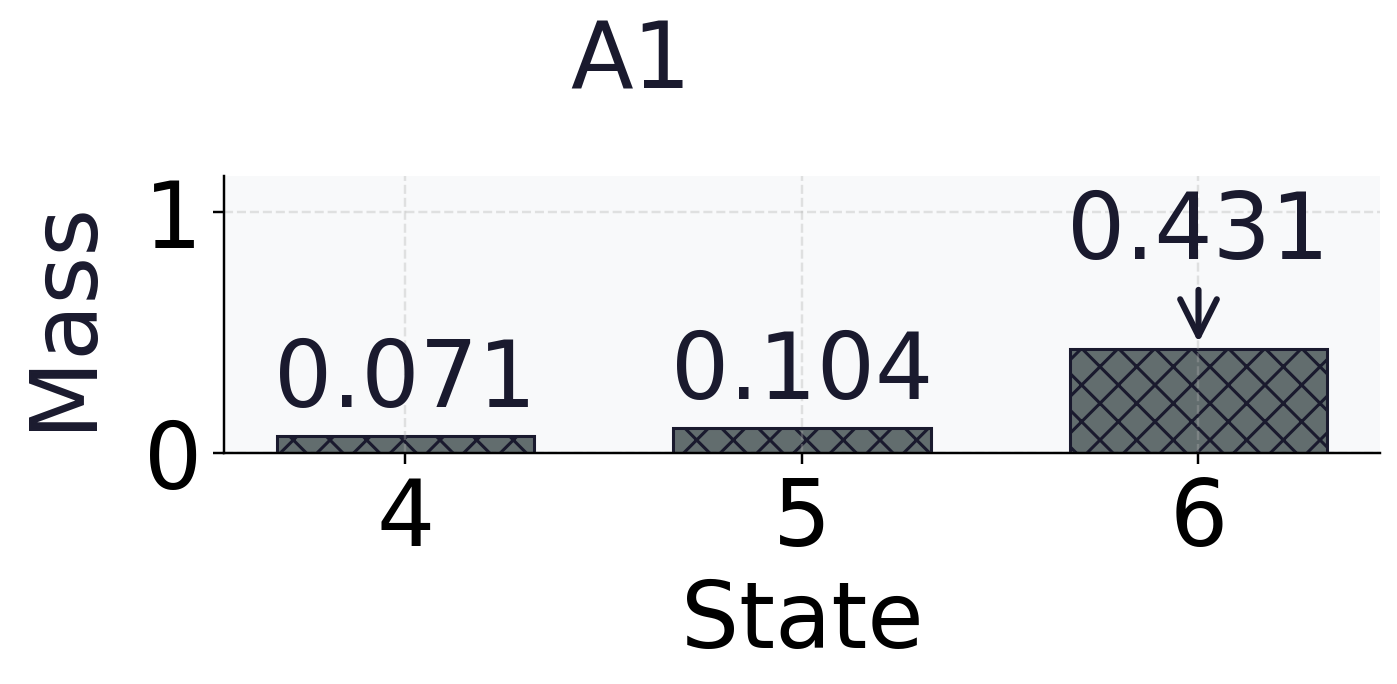
\includegraphics[keepaspectratio,width=0.98\linewidth,height=0.8\textheight,alt={A1: source-derived posterior masses for states 4 to 6, common 0--1 probability scale; arrow marks this row\textquotesingle s argmax when present.}]{../figures/graphical_abstract.slide-row-1-states-4-6.png}
\refstepcounter{figure}\label{fig:graphical-abstract-slide-panel-2}
\end{figure}
\end{frame}

\begin{frame}{Abstract (part 15)}
\begin{figure}
\centering
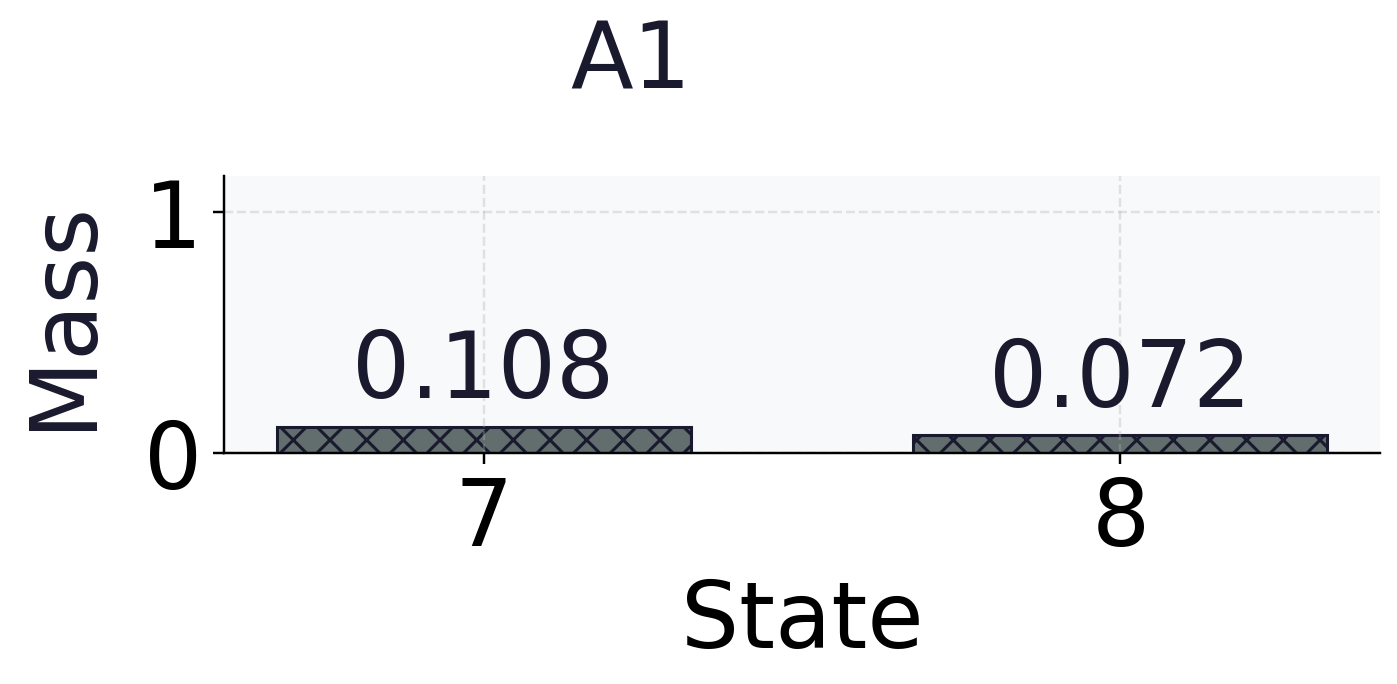
\includegraphics[keepaspectratio,width=0.98\linewidth,height=0.8\textheight,alt={A1: source-derived posterior masses for states 7 to 8, common 0--1 probability scale; arrow marks this row\textquotesingle s argmax when present.}]{../figures/graphical_abstract.slide-row-1-states-7-8.png}
\refstepcounter{figure}\label{fig:graphical-abstract-slide-panel-3}
\end{figure}
\end{frame}

\begin{frame}{Abstract (part 16)}
\begin{figure}
\centering
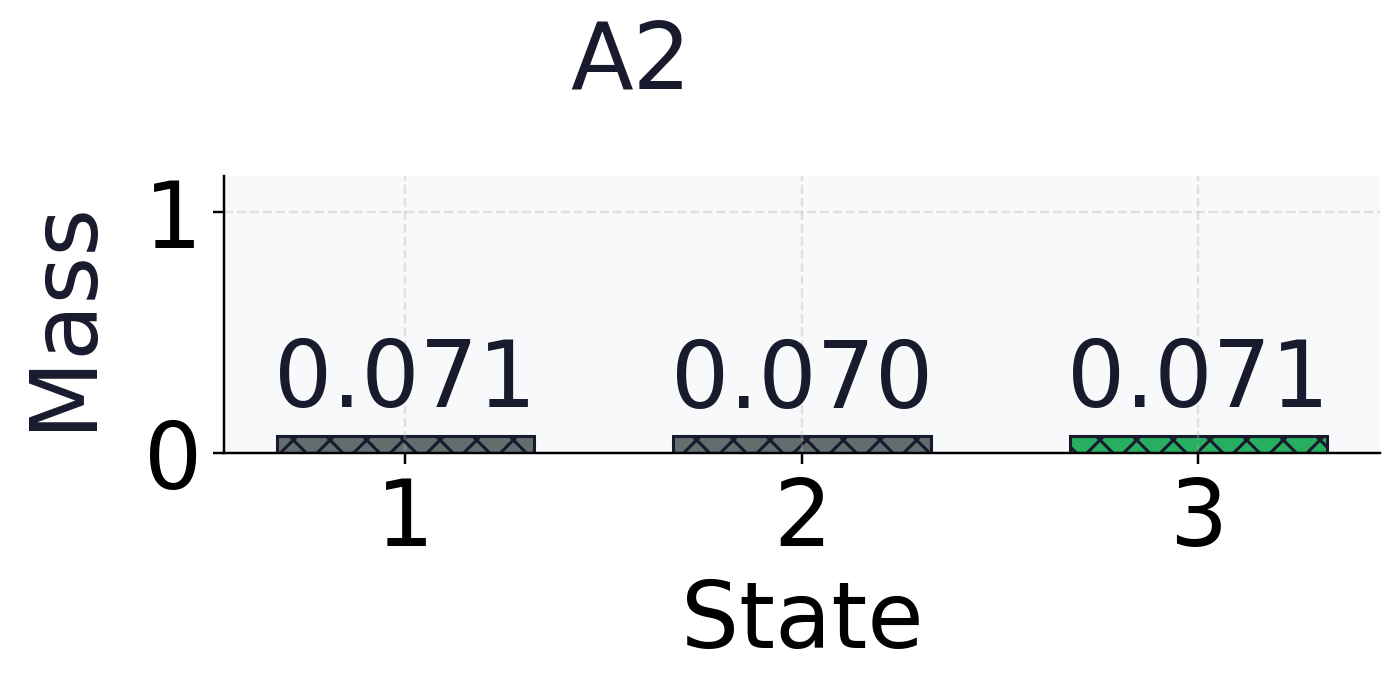
\includegraphics[keepaspectratio,width=0.98\linewidth,height=0.8\textheight,alt={A2: source-derived posterior masses for states 1 to 3, common 0--1 probability scale; arrow marks this row\textquotesingle s argmax when present.}]{../figures/graphical_abstract.slide-row-2-states-1-3.png}
\refstepcounter{figure}\label{fig:graphical-abstract-slide-panel-4}
\end{figure}
\end{frame}

\begin{frame}{Abstract (part 17)}
\begin{figure}
\centering
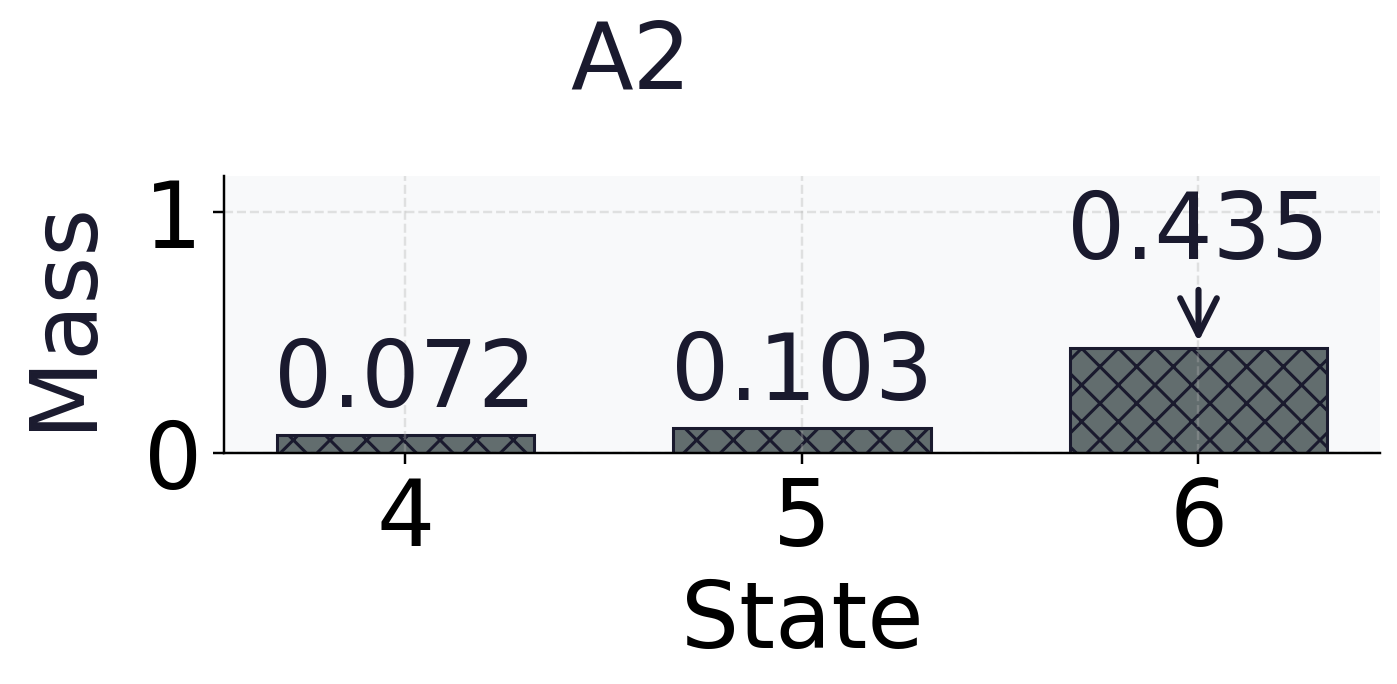
\includegraphics[keepaspectratio,width=0.98\linewidth,height=0.8\textheight,alt={A2: source-derived posterior masses for states 4 to 6, common 0--1 probability scale; arrow marks this row\textquotesingle s argmax when present.}]{../figures/graphical_abstract.slide-row-2-states-4-6.png}
\refstepcounter{figure}\label{fig:graphical-abstract-slide-panel-5}
\end{figure}
\end{frame}

\begin{frame}{Abstract (part 18)}
\begin{figure}
\centering
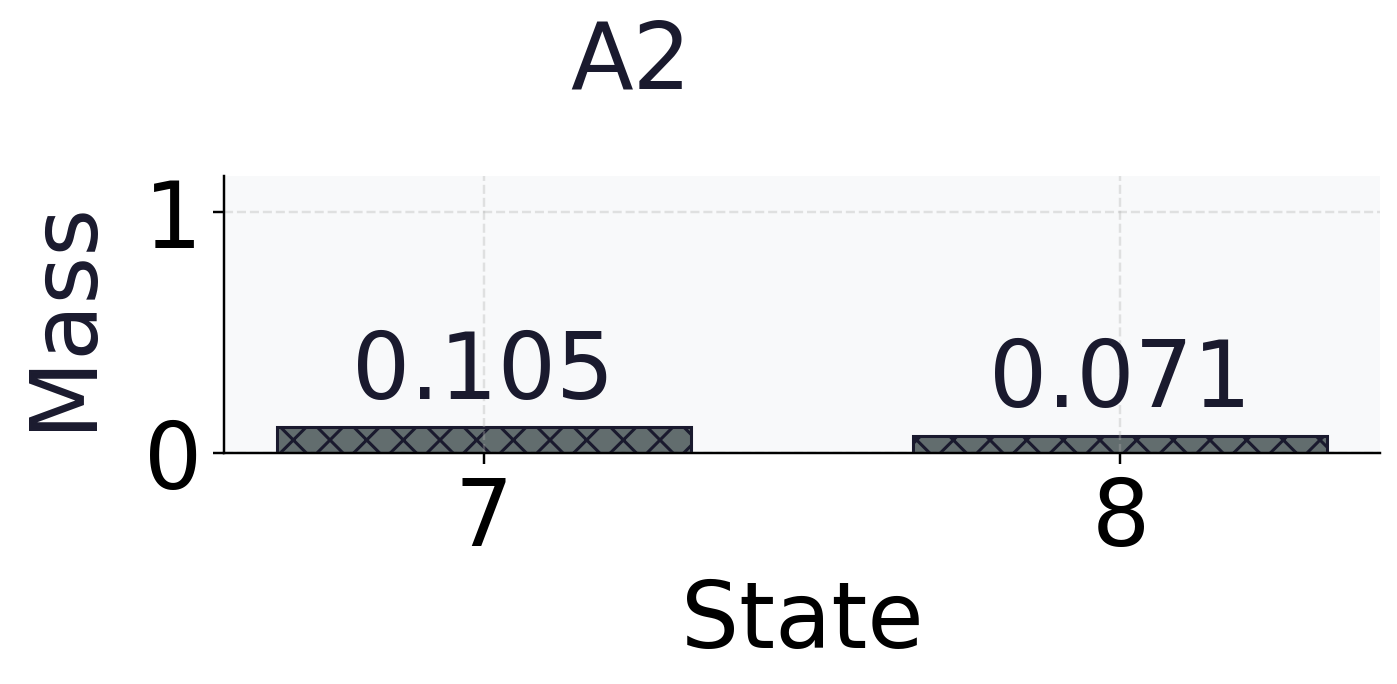
\includegraphics[keepaspectratio,width=0.98\linewidth,height=0.8\textheight,alt={A2: source-derived posterior masses for states 7 to 8, common 0--1 probability scale; arrow marks this row\textquotesingle s argmax when present.}]{../figures/graphical_abstract.slide-row-2-states-7-8.png}
\refstepcounter{figure}\label{fig:graphical-abstract-slide-panel-6}
\end{figure}
\end{frame}

\begin{frame}{Abstract (part 19)}
\begin{figure}
\centering
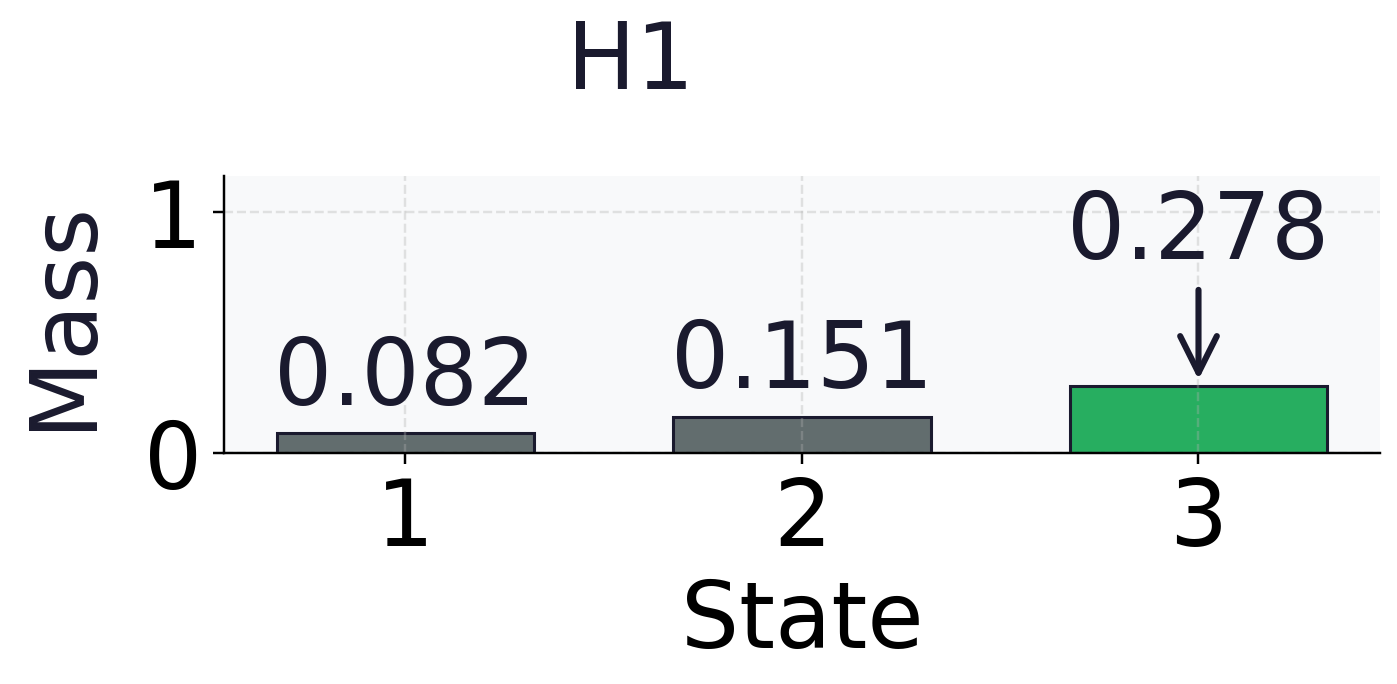
\includegraphics[keepaspectratio,width=0.98\linewidth,height=0.8\textheight,alt={H1: source-derived posterior masses for states 1 to 3, common 0--1 probability scale; arrow marks this row\textquotesingle s argmax when present.}]{../figures/graphical_abstract.slide-row-3-states-1-3.png}
\refstepcounter{figure}\label{fig:graphical-abstract-slide-panel-7}
\end{figure}
\end{frame}

\begin{frame}{Abstract (part 20)}
\begin{figure}
\centering
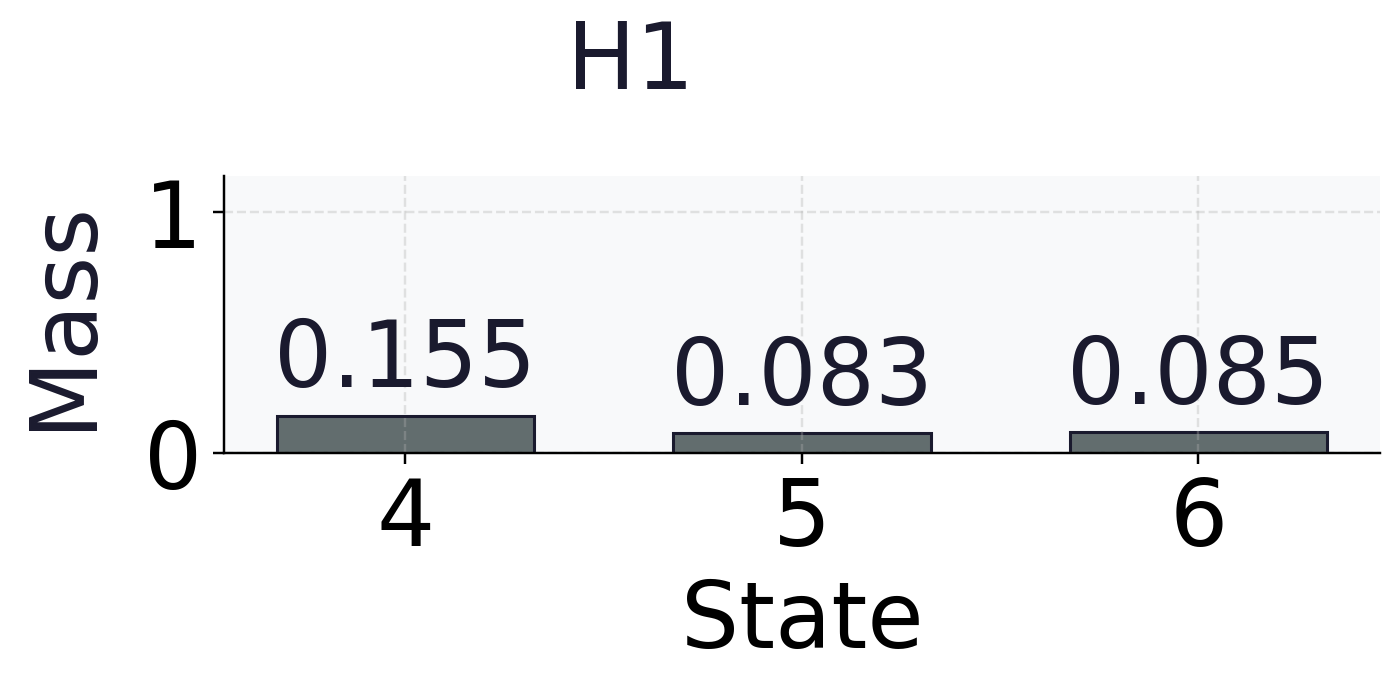
\includegraphics[keepaspectratio,width=0.98\linewidth,height=0.8\textheight,alt={H1: source-derived posterior masses for states 4 to 6, common 0--1 probability scale; arrow marks this row\textquotesingle s argmax when present.}]{../figures/graphical_abstract.slide-row-3-states-4-6.png}
\refstepcounter{figure}\label{fig:graphical-abstract-slide-panel-8}
\end{figure}
\end{frame}

\begin{frame}{Abstract (part 21)}
\begin{figure}
\centering
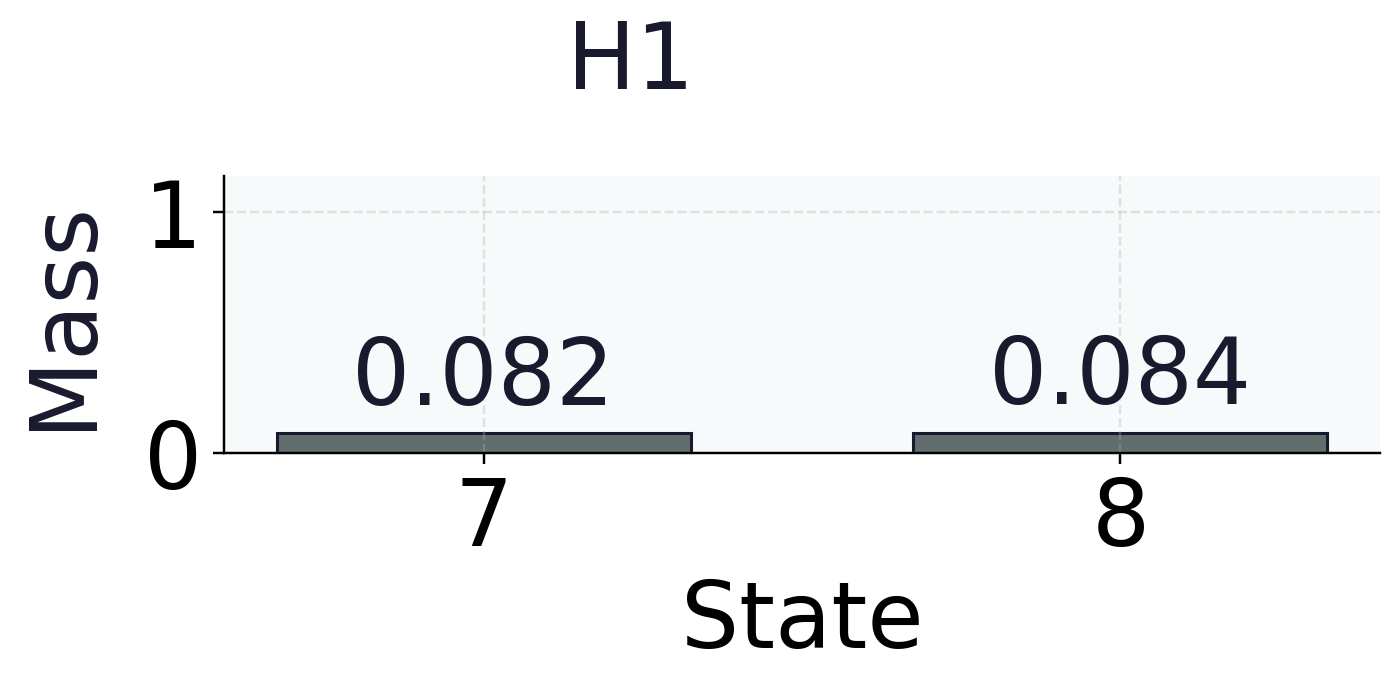
\includegraphics[keepaspectratio,width=0.98\linewidth,height=0.8\textheight,alt={H1: source-derived posterior masses for states 7 to 8, common 0--1 probability scale; arrow marks this row\textquotesingle s argmax when present.}]{../figures/graphical_abstract.slide-row-3-states-7-8.png}
\refstepcounter{figure}\label{fig:graphical-abstract-slide-panel-9}
\end{figure}
\end{frame}

\begin{frame}{Abstract (part 22)}
\begin{figure}
\centering
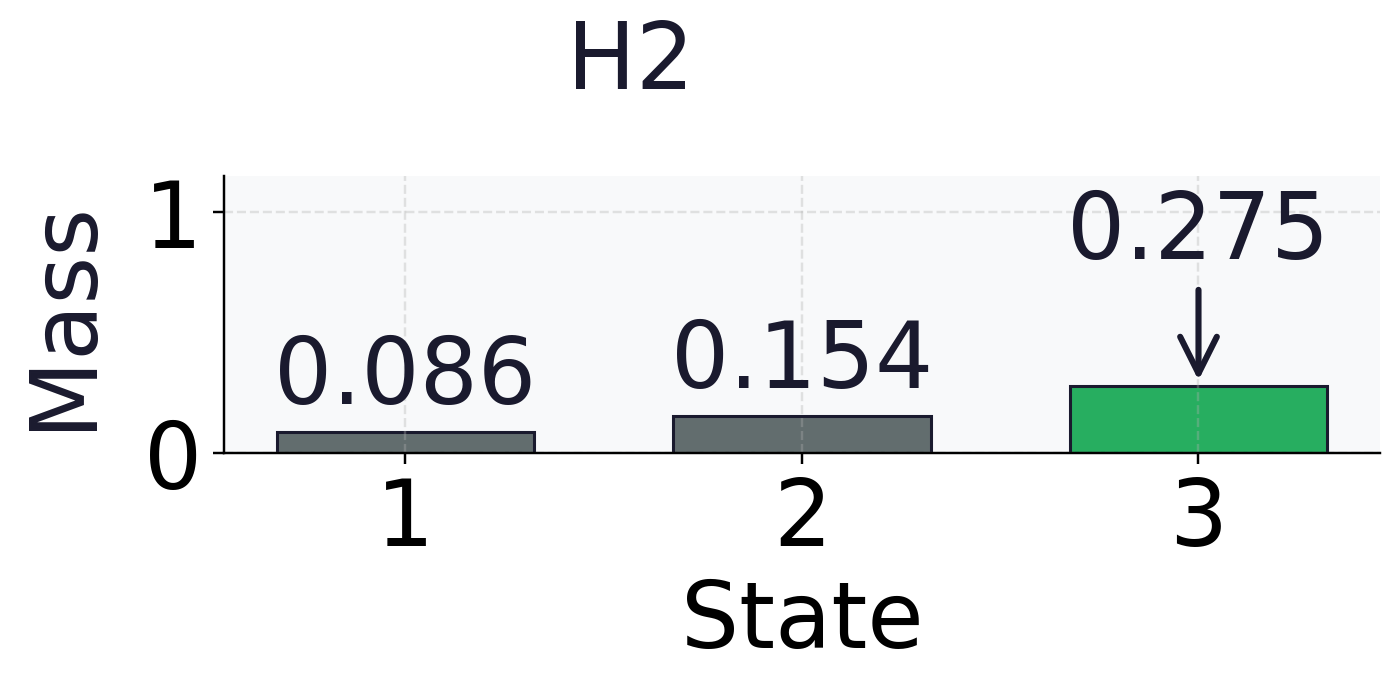
\includegraphics[keepaspectratio,width=0.98\linewidth,height=0.8\textheight,alt={H2: source-derived posterior masses for states 1 to 3, common 0--1 probability scale; arrow marks this row\textquotesingle s argmax when present.}]{../figures/graphical_abstract.slide-row-4-states-1-3.png}
\refstepcounter{figure}\label{fig:graphical-abstract-slide-panel-10}
\end{figure}
\end{frame}

\begin{frame}{Abstract (part 23)}
\begin{figure}
\centering
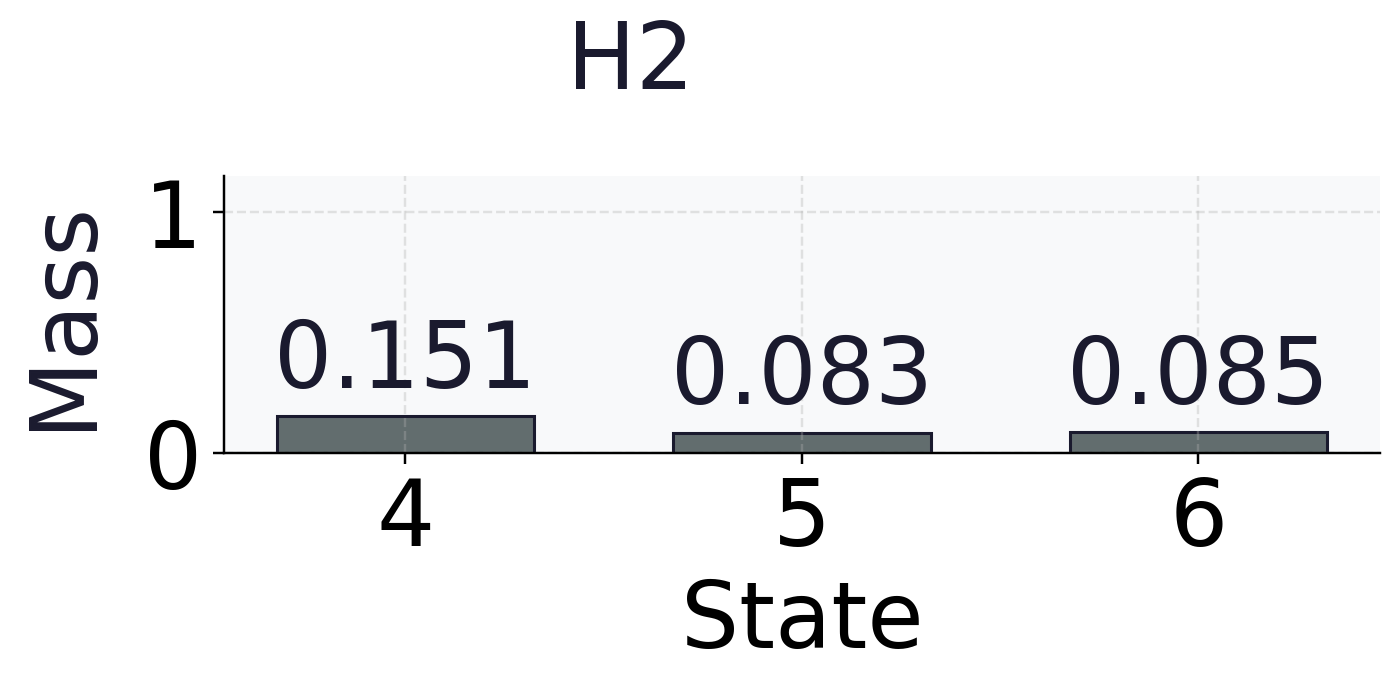
\includegraphics[keepaspectratio,width=0.98\linewidth,height=0.8\textheight,alt={H2: source-derived posterior masses for states 4 to 6, common 0--1 probability scale; arrow marks this row\textquotesingle s argmax when present.}]{../figures/graphical_abstract.slide-row-4-states-4-6.png}
\refstepcounter{figure}\label{fig:graphical-abstract-slide-panel-11}
\end{figure}
\end{frame}

\begin{frame}{Abstract (part 24)}
\begin{figure}
\centering
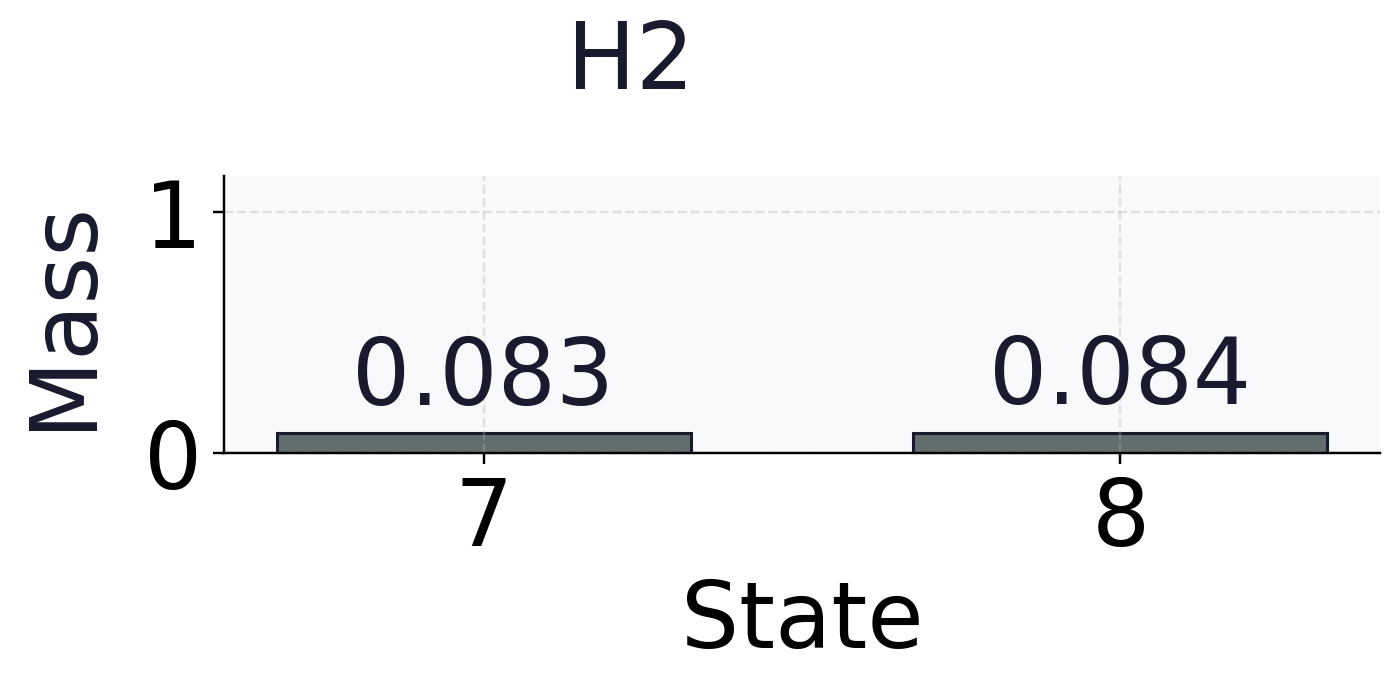
\includegraphics[keepaspectratio,width=0.98\linewidth,height=0.8\textheight,alt={H2: source-derived posterior masses for states 7 to 8, common 0--1 probability scale; arrow marks this row\textquotesingle s argmax when present.}]{../figures/graphical_abstract.slide-row-4-states-7-8.png}
\refstepcounter{figure}\label{fig:graphical-abstract-slide-panel-12}
\end{figure}
\end{frame}

\begin{frame}{Abstract (part 25)}
\begin{figure}
\centering
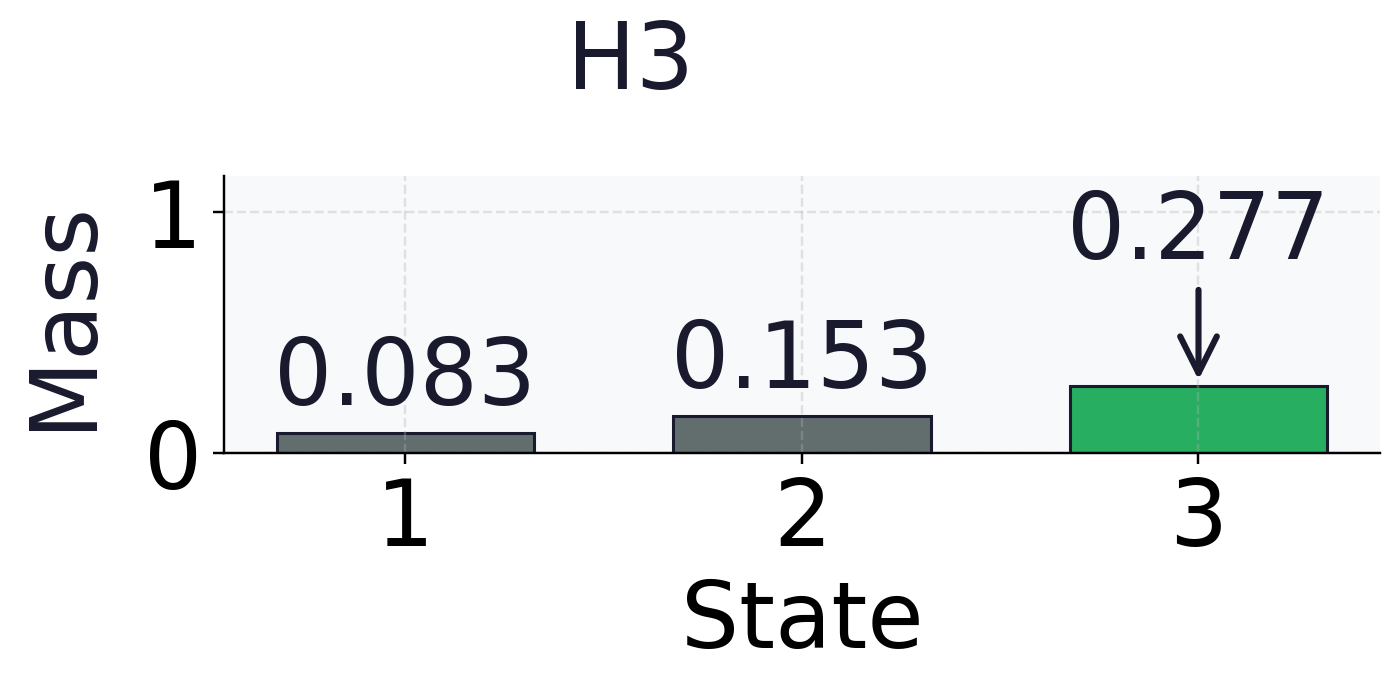
\includegraphics[keepaspectratio,width=0.98\linewidth,height=0.8\textheight,alt={H3: source-derived posterior masses for states 1 to 3, common 0--1 probability scale; arrow marks this row\textquotesingle s argmax when present.}]{../figures/graphical_abstract.slide-row-5-states-1-3.png}
\refstepcounter{figure}\label{fig:graphical-abstract-slide-panel-13}
\end{figure}
\end{frame}

\begin{frame}{Abstract (part 26)}
\begin{figure}
\centering
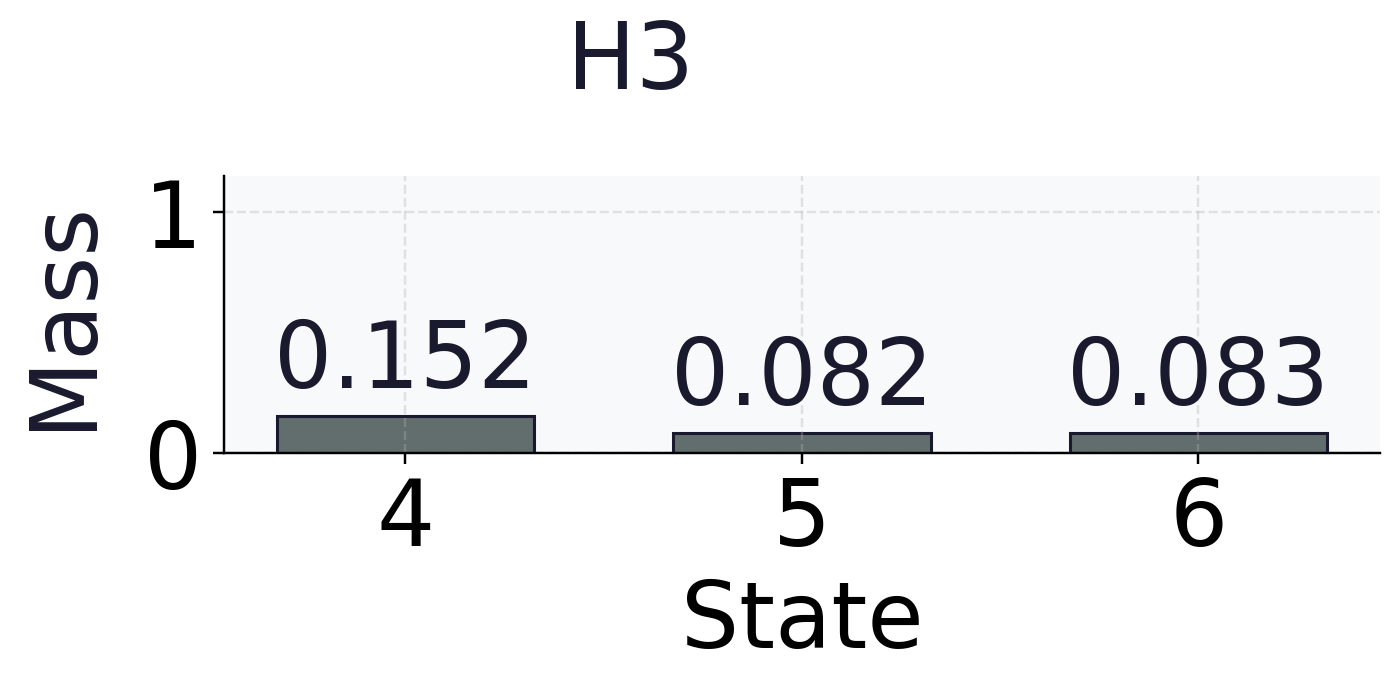
\includegraphics[keepaspectratio,width=0.98\linewidth,height=0.8\textheight,alt={H3: source-derived posterior masses for states 4 to 6, common 0--1 probability scale; arrow marks this row\textquotesingle s argmax when present.}]{../figures/graphical_abstract.slide-row-5-states-4-6.png}
\refstepcounter{figure}\label{fig:graphical-abstract-slide-panel-14}
\end{figure}
\end{frame}

\begin{frame}{Abstract (part 27)}
\begin{figure}
\centering
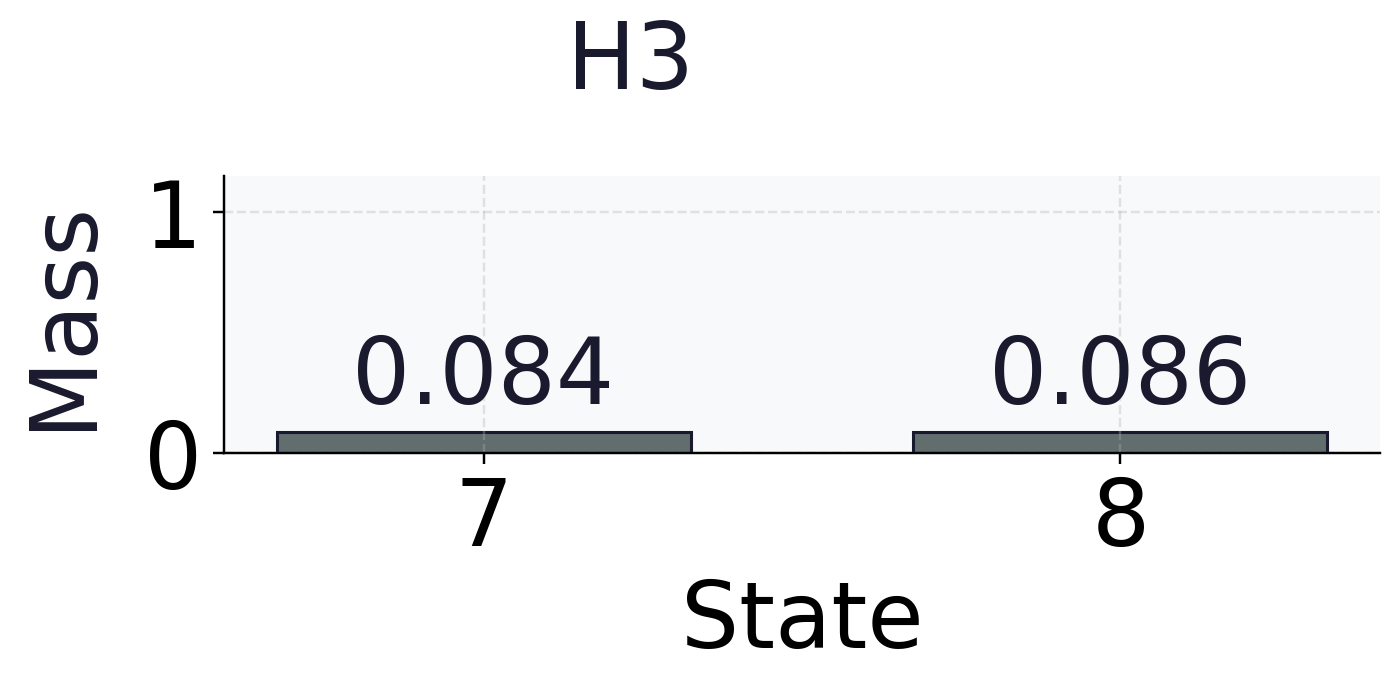
\includegraphics[keepaspectratio,width=0.98\linewidth,height=0.8\textheight,alt={H3: source-derived posterior masses for states 7 to 8, common 0--1 probability scale; arrow marks this row\textquotesingle s argmax when present.}]{../figures/graphical_abstract.slide-row-5-states-7-8.png}
\refstepcounter{figure}\label{fig:graphical-abstract-slide-panel-15}
\end{figure}
\end{frame}

\begin{frame}{Abstract (part 28)}
\begin{figure}
\centering
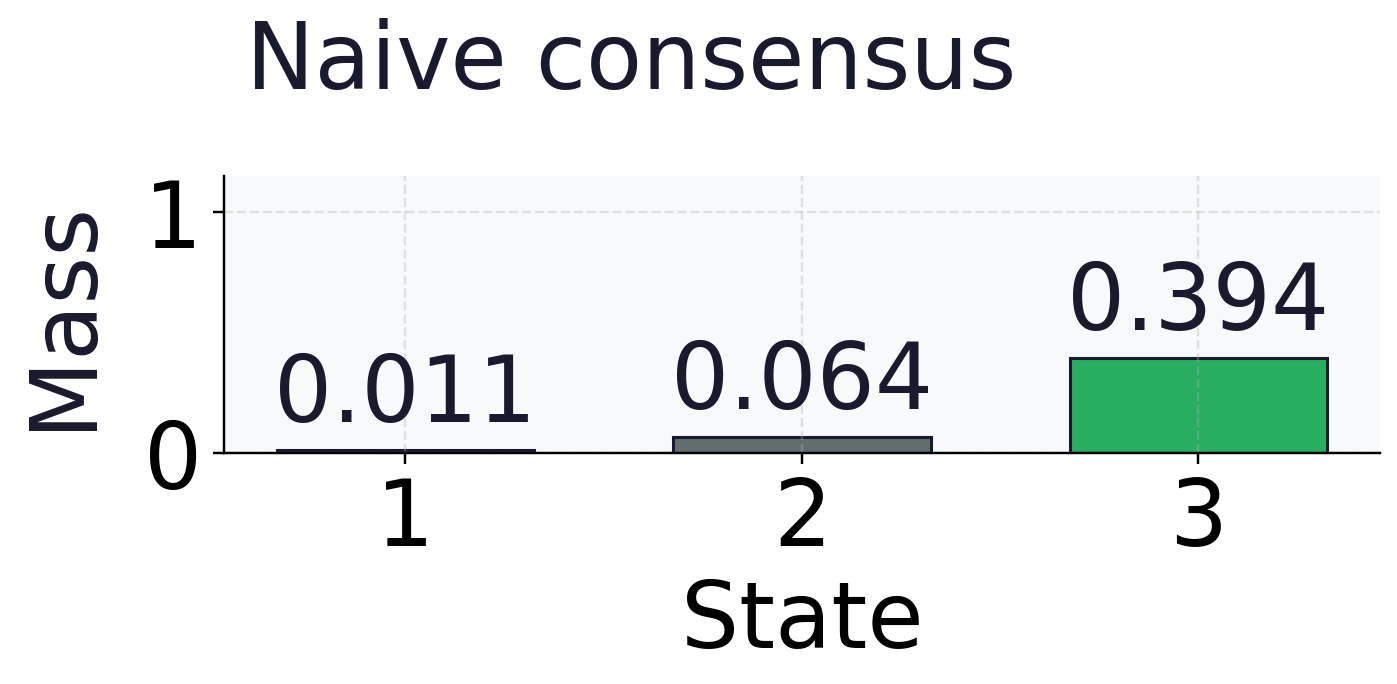
\includegraphics[keepaspectratio,width=0.98\linewidth,height=0.8\textheight,alt={Naive consensus: source-derived posterior masses for states 1 to 3, common 0--1 probability scale; arrow marks this row\textquotesingle s argmax when present.}]{../figures/graphical_abstract.slide-row-6-states-1-3.png}
\refstepcounter{figure}\label{fig:graphical-abstract-slide-panel-16}
\end{figure}
\end{frame}

\begin{frame}{Abstract (part 29)}
\begin{figure}
\centering
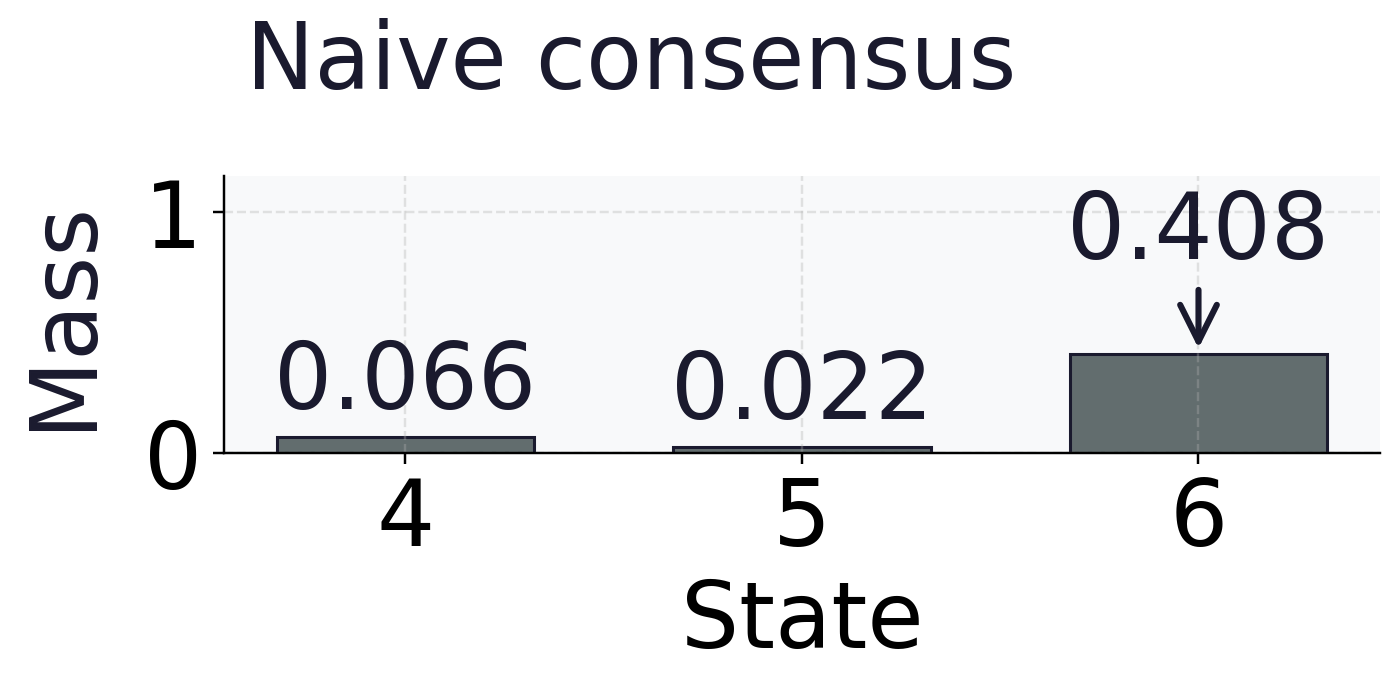
\includegraphics[keepaspectratio,width=0.98\linewidth,height=0.8\textheight,alt={Naive consensus: source-derived posterior masses for states 4 to 6, common 0--1 probability scale; arrow marks this row\textquotesingle s argmax when present.}]{../figures/graphical_abstract.slide-row-6-states-4-6.png}
\refstepcounter{figure}\label{fig:graphical-abstract-slide-panel-17}
\end{figure}
\end{frame}

\begin{frame}{Abstract (part 30)}
\begin{figure}
\centering
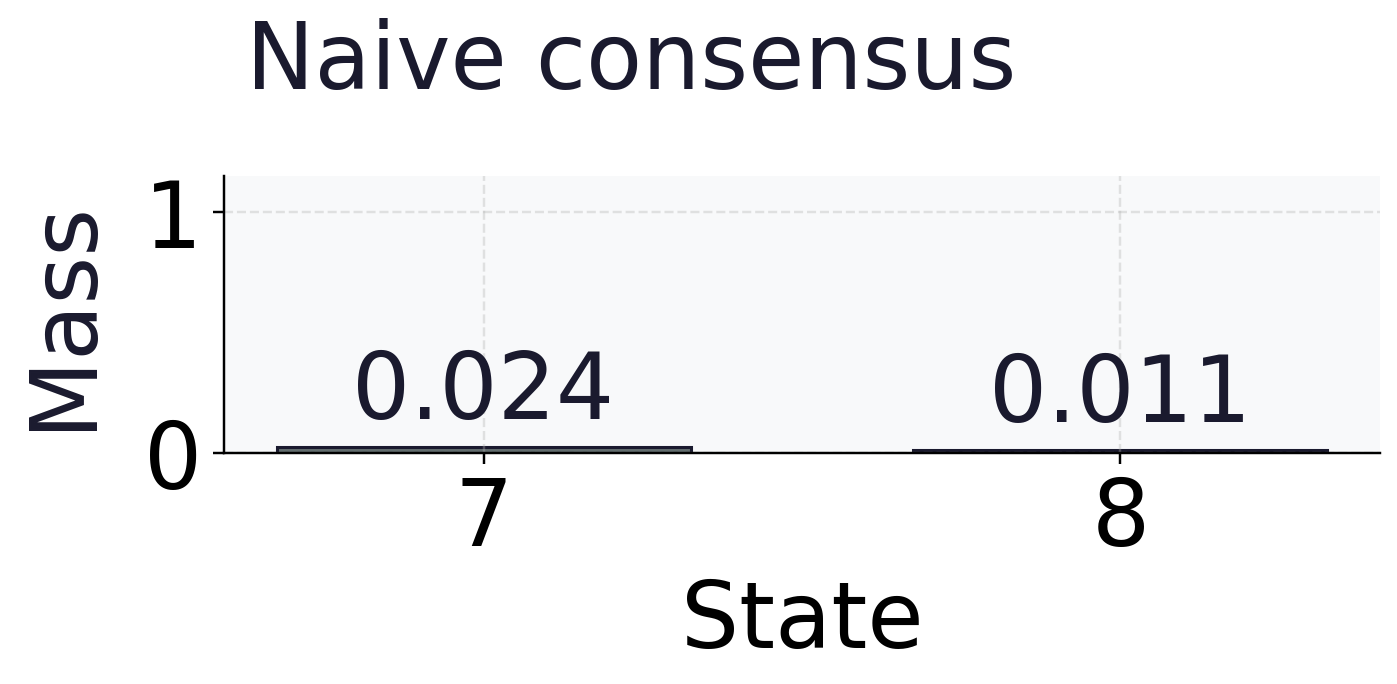
\includegraphics[keepaspectratio,width=0.98\linewidth,height=0.8\textheight,alt={Naive consensus: source-derived posterior masses for states 7 to 8, common 0--1 probability scale; arrow marks this row\textquotesingle s argmax when present.}]{../figures/graphical_abstract.slide-row-6-states-7-8.png}
\refstepcounter{figure}\label{fig:graphical-abstract-slide-panel-18}
\end{figure}
\end{frame}

\begin{frame}{Abstract (part 31)}
\begin{figure}
\centering
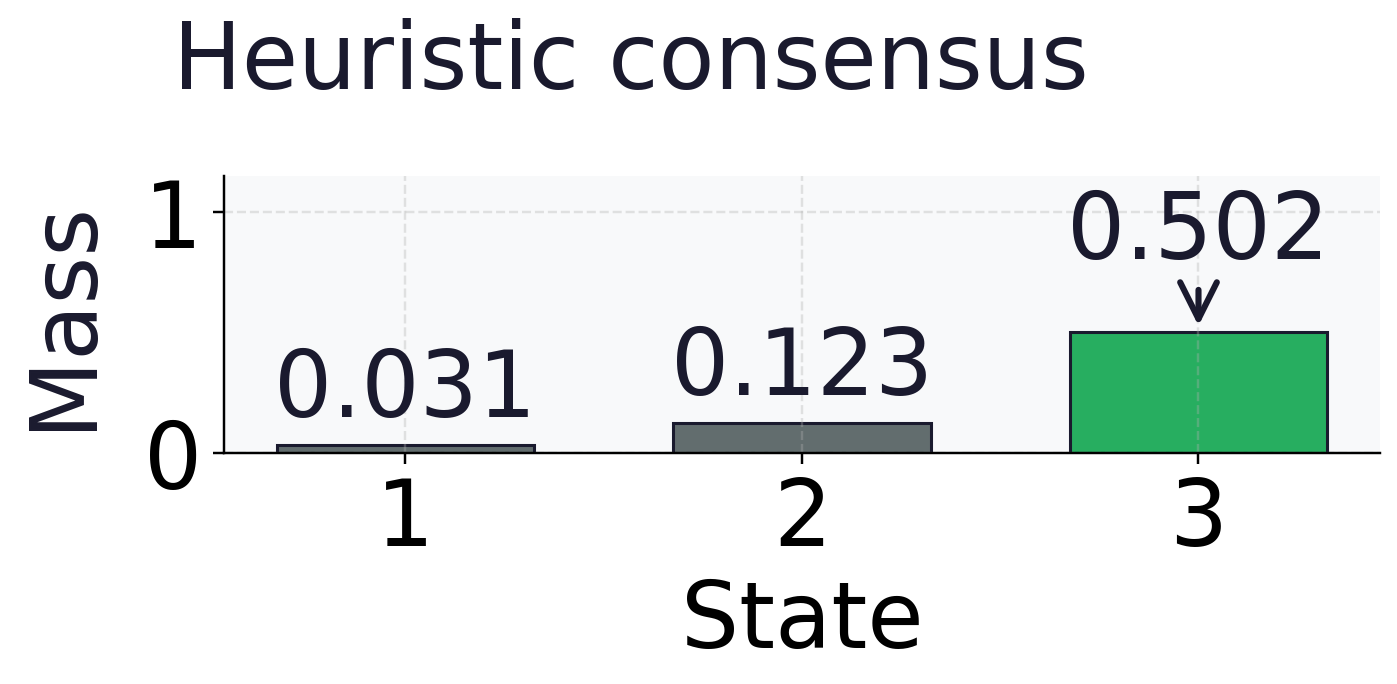
\includegraphics[keepaspectratio,width=0.98\linewidth,height=0.8\textheight,alt={Heuristic consensus: source-derived posterior masses for states 1 to 3, common 0--1 probability scale; arrow marks this row\textquotesingle s argmax when present.}]{../figures/graphical_abstract.slide-row-7-states-1-3.png}
\refstepcounter{figure}\label{fig:graphical-abstract-slide-panel-19}
\end{figure}
\end{frame}

\begin{frame}{Abstract (part 32)}
\begin{figure}
\centering
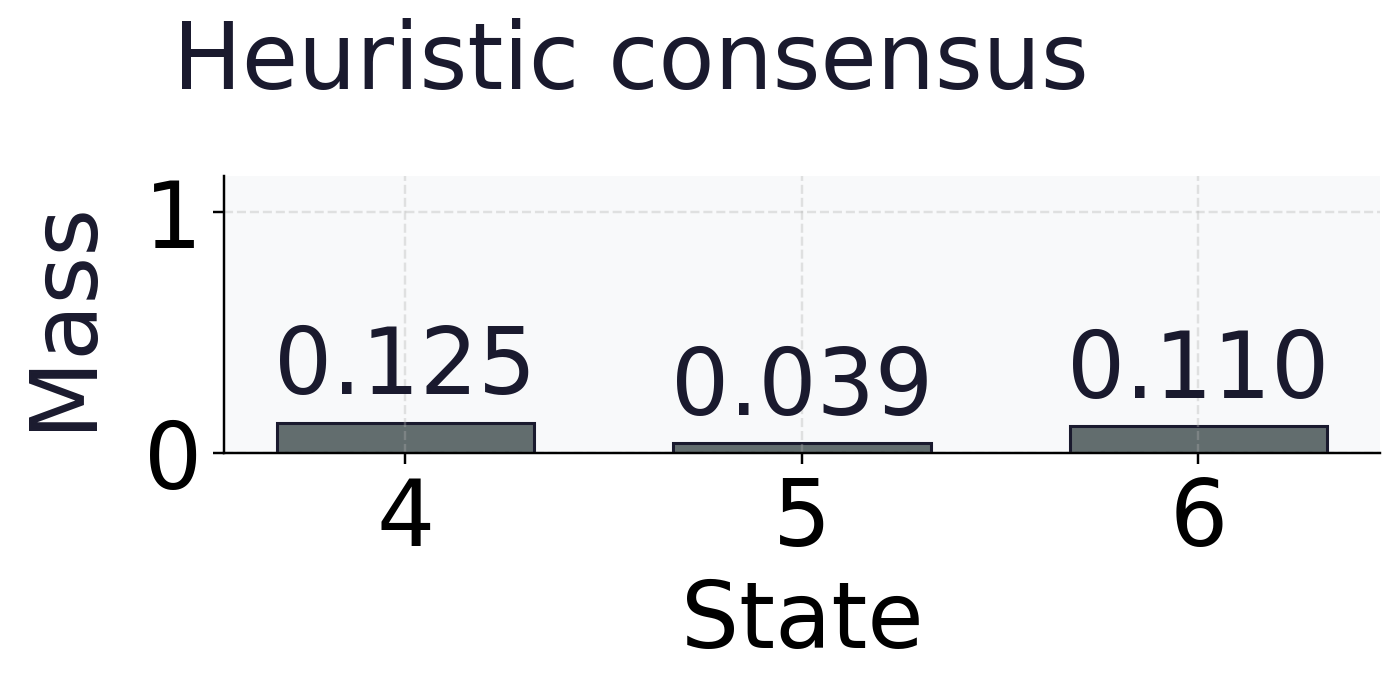
\includegraphics[keepaspectratio,width=0.98\linewidth,height=0.8\textheight,alt={Heuristic consensus: source-derived posterior masses for states 4 to 6, common 0--1 probability scale; arrow marks this row\textquotesingle s argmax when present.}]{../figures/graphical_abstract.slide-row-7-states-4-6.png}
\refstepcounter{figure}\label{fig:graphical-abstract-slide-panel-20}
\end{figure}
\end{frame}

\begin{frame}{Abstract (part 33)}
\begin{figure}
\centering
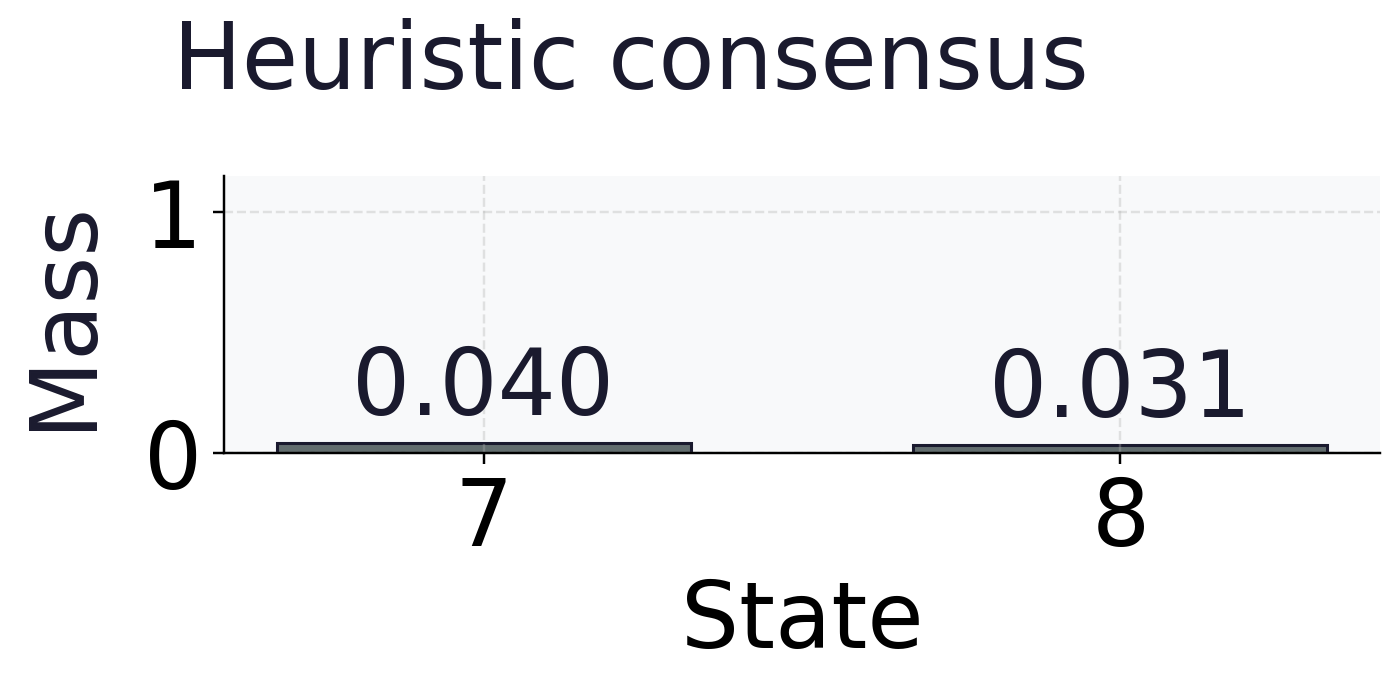
\includegraphics[keepaspectratio,width=0.98\linewidth,height=0.8\textheight,alt={Heuristic consensus: source-derived posterior masses for states 7 to 8, common 0--1 probability scale; arrow marks this row\textquotesingle s argmax when present.}]{../figures/graphical_abstract.slide-row-7-states-7-8.png}
\refstepcounter{figure}\label{fig:graphical-abstract-slide-panel-21}
\end{figure}
\end{frame}

\begin{frame}{Abstract (part 34)}
\begin{figure}
\centering
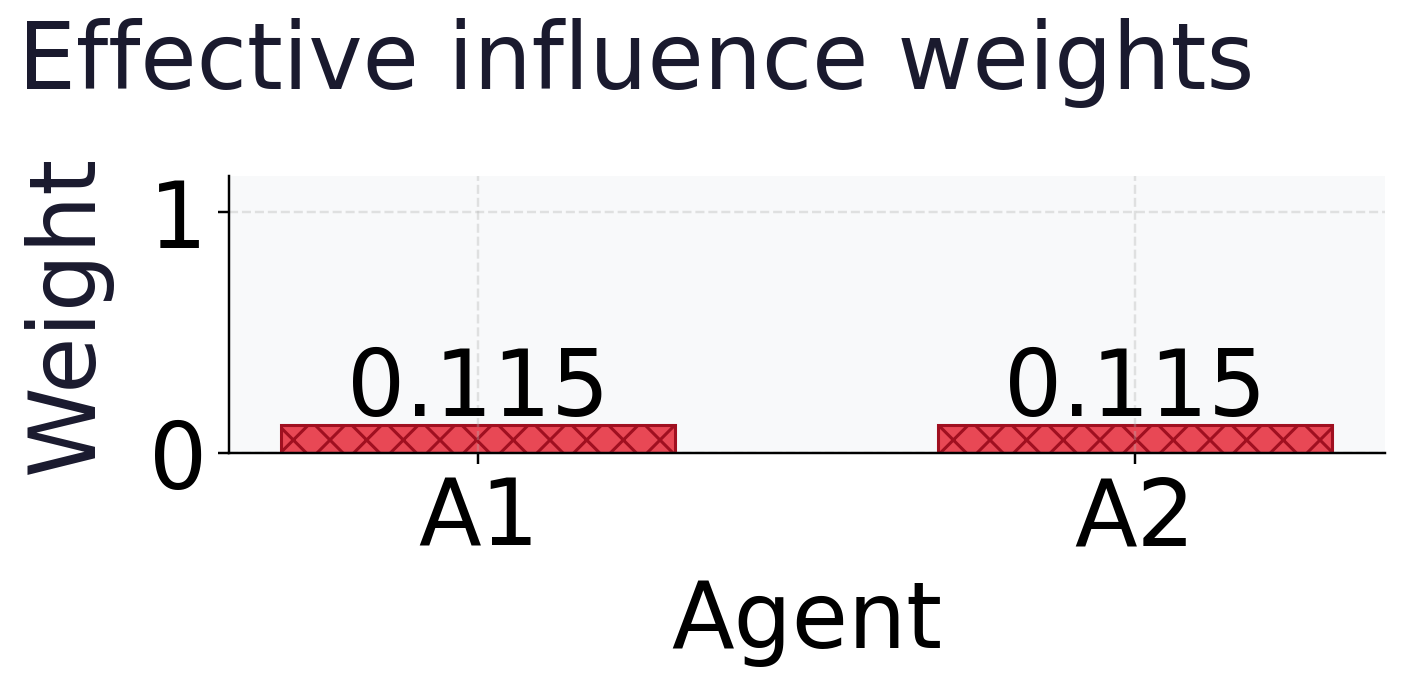
\includegraphics[keepaspectratio,width=0.98\linewidth,height=0.8\textheight,alt={Source-derived normalized heuristic influence weights; adversarial bars are crosshatched and agent labels preserve their roles.}]{../figures/graphical_abstract.slide-weights-1-2.png}
\refstepcounter{figure}\label{fig:graphical-abstract-slide-panel-22}
\end{figure}
\end{frame}

\begin{frame}{Abstract (part 35)}
\begin{figure}
\centering
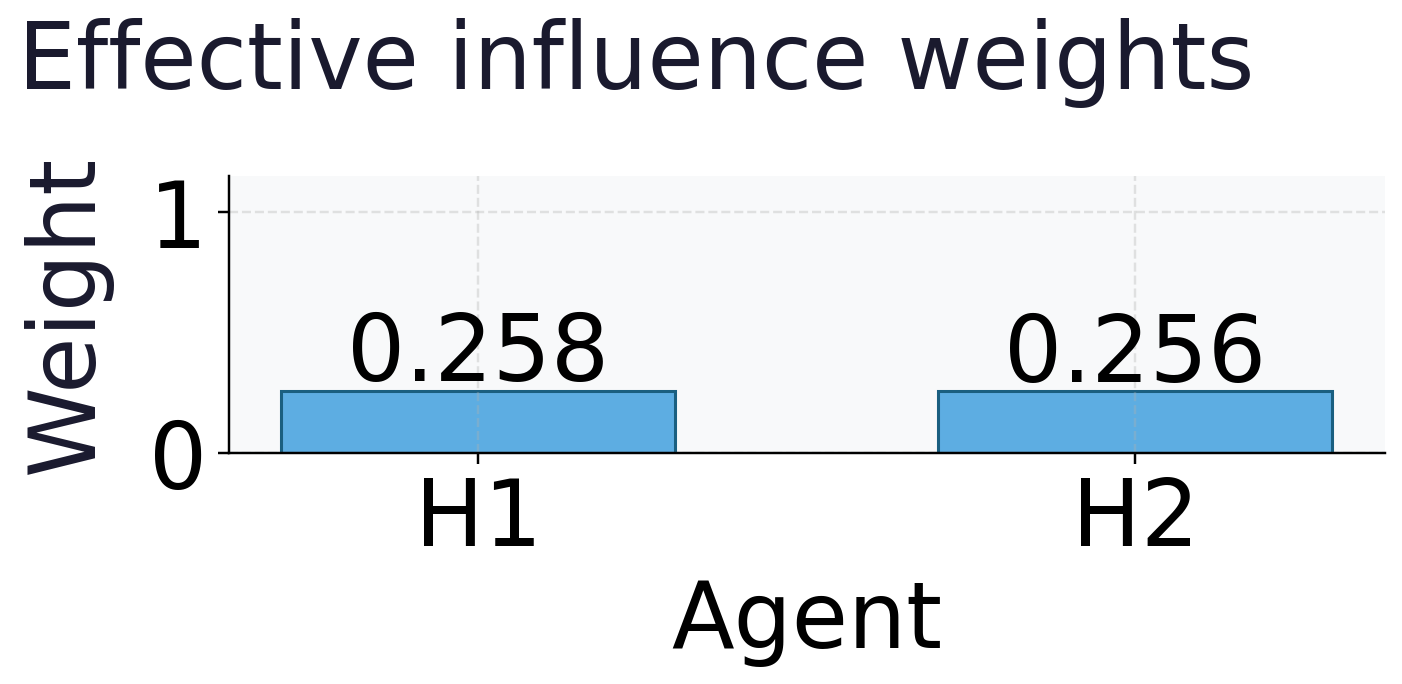
\includegraphics[keepaspectratio,width=0.98\linewidth,height=0.8\textheight,alt={Source-derived normalized heuristic influence weights; adversarial bars are crosshatched and agent labels preserve their roles.}]{../figures/graphical_abstract.slide-weights-3-4.png}
\refstepcounter{figure}\label{fig:graphical-abstract-slide-panel-23}
\end{figure}
\end{frame}

\begin{frame}{Abstract (part 36)}
\begin{figure}
\centering
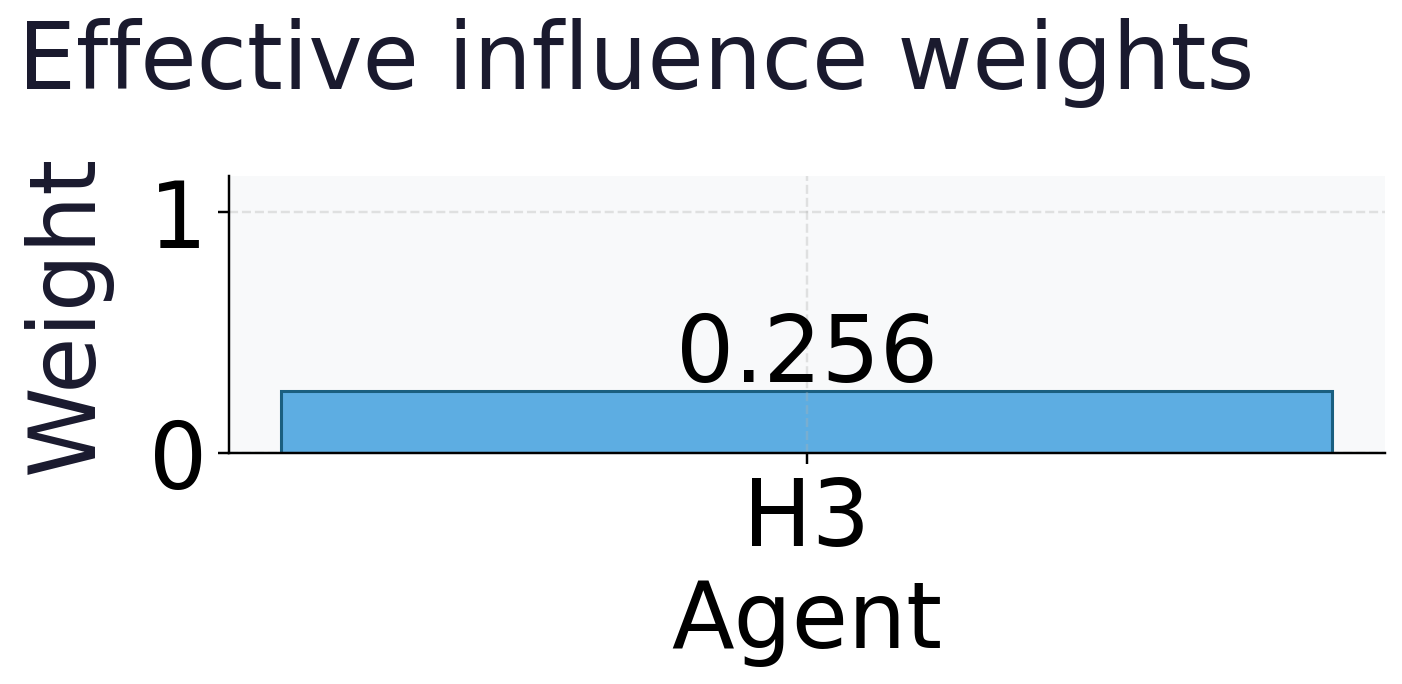
\includegraphics[keepaspectratio,width=0.98\linewidth,height=0.8\textheight,alt={Source-derived normalized heuristic influence weights; adversarial bars are crosshatched and agent labels preserve their roles.}]{../figures/graphical_abstract.slide-weights-5-5.png}
\refstepcounter{figure}\label{fig:graphical-abstract-slide-panel-24}
\end{figure}
\end{frame}

\begin{frame}{Abstract (part 37)}
\begin{figure}
\centering
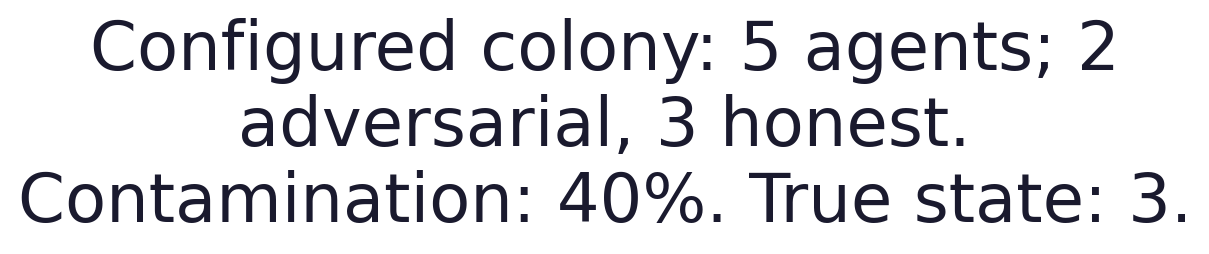
\includegraphics[keepaspectratio,width=0.98\linewidth,height=0.8\textheight,alt={Configured colony: 5 agents; 2 adversarial, 3 honest. Contamination: 40\%. True state: 3.}]{../figures/graphical_abstract.slide-colony.png}
\refstepcounter{figure}\label{fig:graphical-abstract-slide-panel-25}
\end{figure}
\end{frame}

\begin{frame}{Abstract (part 38)}
\begin{figure}
\centering

\includegraphics[keepaspectratio,width=0.98\linewidth,height=0.8\textheight,alt={Naive equal-weight log pool: true-state mass 39\%; argmax state 6.}]{../figures/graphical_abstract.slide-naive.png}
\refstepcounter{figure}\label{fig:graphical-abstract-slide-panel-26}
\end{figure}
\end{frame}

\begin{frame}{Abstract (part 39)}
\begin{figure}
\centering
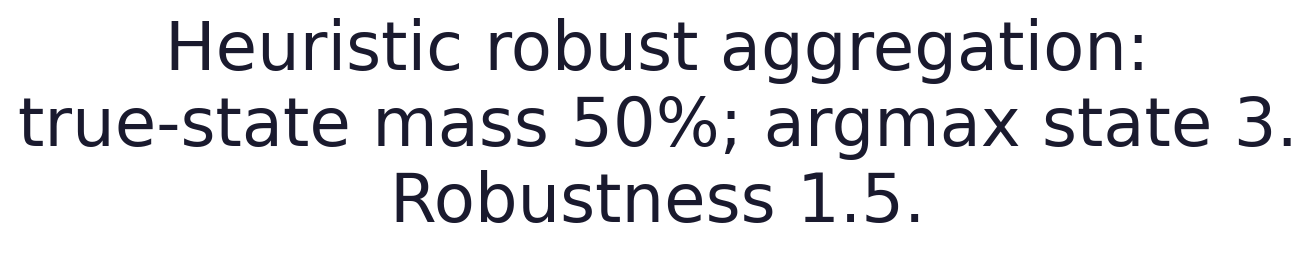
\includegraphics[keepaspectratio,width=0.98\linewidth,height=0.8\textheight,alt={Heuristic robust aggregation: true-state mass 50\%; argmax state 3. Robustness 1.5.}]{../figures/graphical_abstract.slide-heuristic.png}
\refstepcounter{figure}\label{fig:graphical-abstract-slide-panel-27}
\end{figure}
\end{frame}

\begin{frame}{Abstract (part 40)}
\begin{figure}
\centering
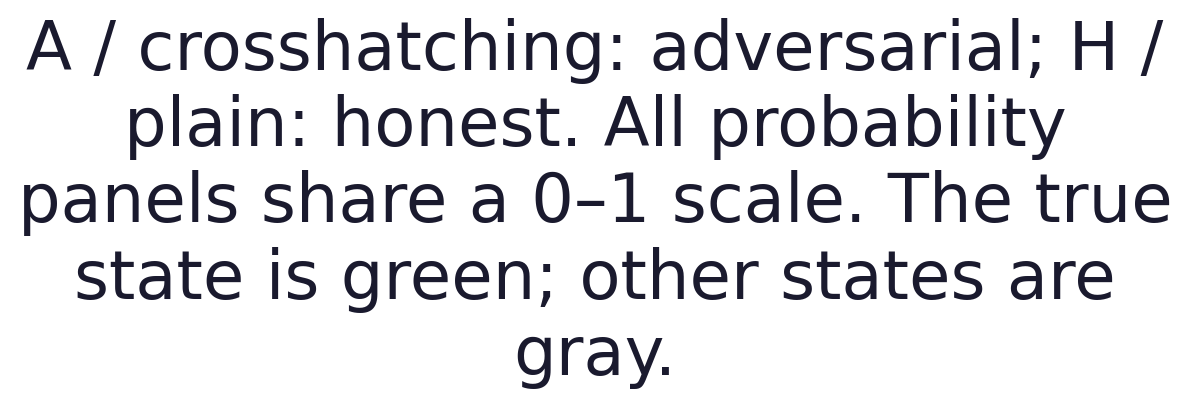
\includegraphics[keepaspectratio,width=0.98\linewidth,height=0.8\textheight,alt={A / crosshatching: adversarial; H / plain: honest. All probability panels share a 0--1 scale. The true state is green; other states are gray.}]{../figures/graphical_abstract.slide-key.png}
\refstepcounter{figure}\label{fig:graphical-abstract-slide-panel-28}
\end{figure}
\end{frame}

\begin{frame}{Abstract (part 41)}
\begin{figure}
\centering
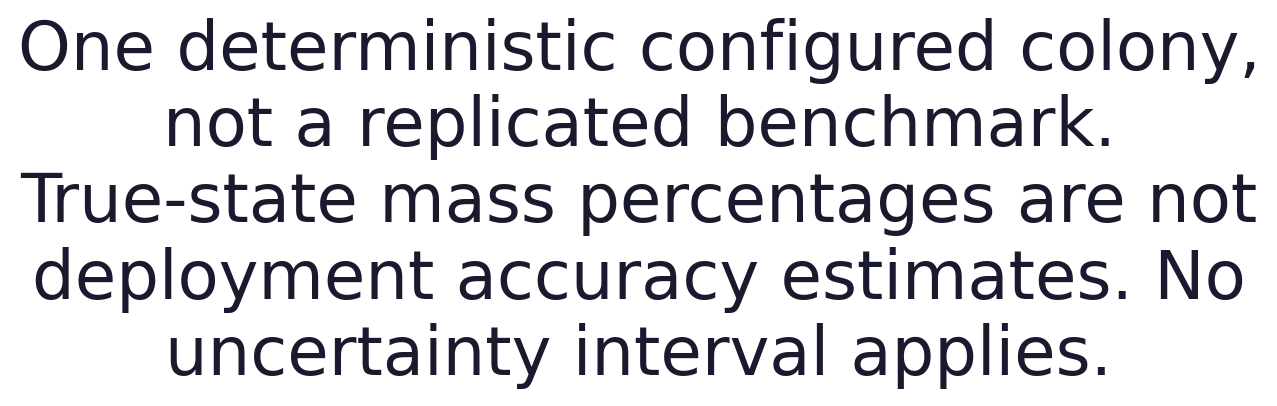
\includegraphics[keepaspectratio,width=0.98\linewidth,height=0.8\textheight,alt={One deterministic configured colony, not a replicated benchmark. True-state mass percentages are not deployment accuracy estimates. No uncertainty interval applies.}]{../figures/graphical_abstract.slide-scope.png}
\refstepcounter{figure}\label{fig:graphical-abstract-slide-panel-29}
\end{figure}
\end{frame}

\begin{frame}{Abstract (part 42)}
\begin{figure}
\centering
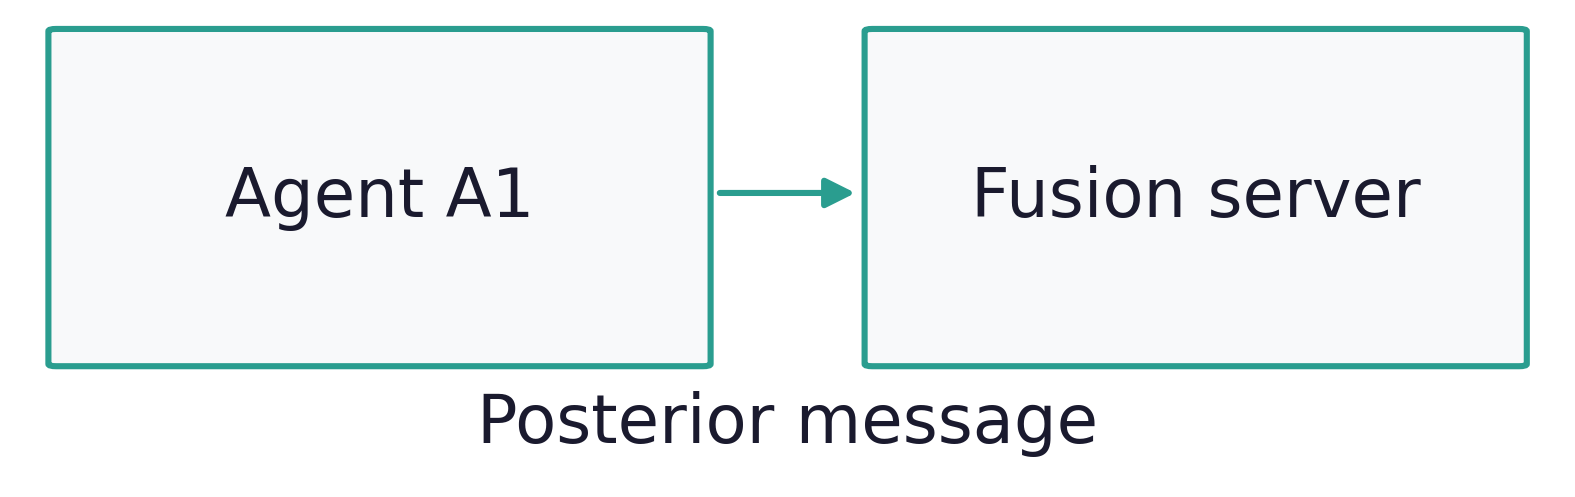
\includegraphics[keepaspectratio,width=0.98\linewidth,height=0.8\textheight,alt={Agent A1 → Fusion server: Posterior message; data\_dependency.}]{../figures/graphical_abstract.slide-network-a1.png}
\refstepcounter{figure}\label{fig:graphical-abstract-slide-panel-30}
\end{figure}
\end{frame}

\begin{frame}{Abstract (part 43)}
\begin{figure}
\centering
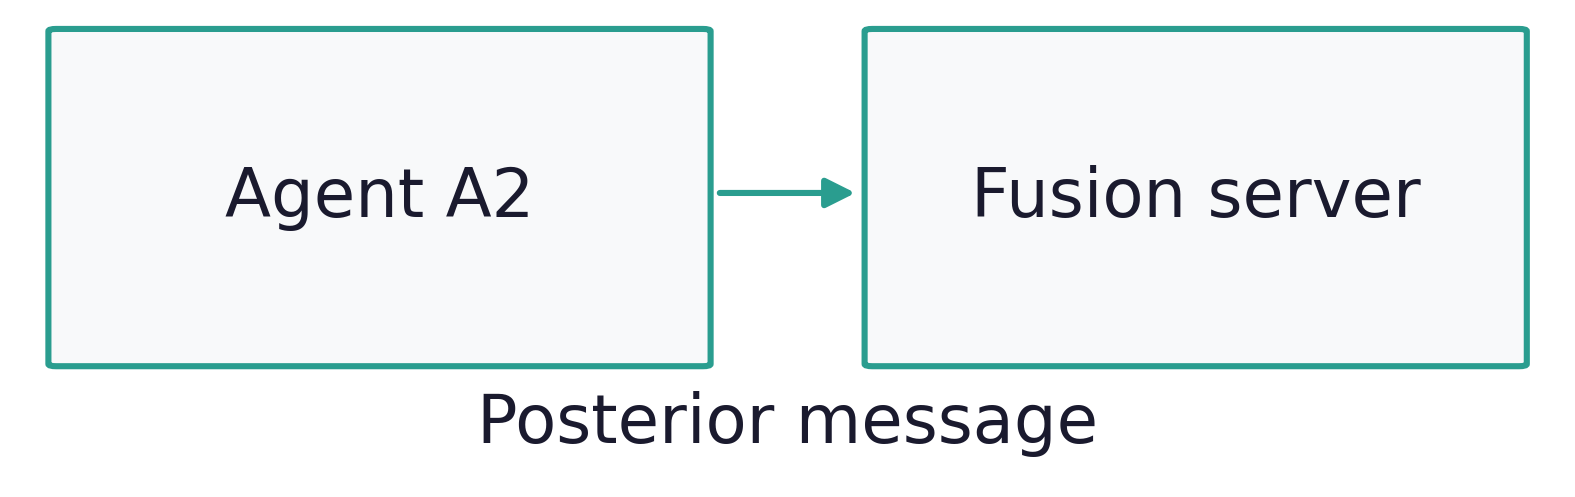
\includegraphics[keepaspectratio,width=0.98\linewidth,height=0.8\textheight,alt={Agent A2 → Fusion server: Posterior message; data\_dependency.}]{../figures/graphical_abstract.slide-network-a2.png}
\refstepcounter{figure}\label{fig:graphical-abstract-slide-panel-31}
\end{figure}
\end{frame}

\begin{frame}{Abstract (part 44)}
\begin{figure}
\centering
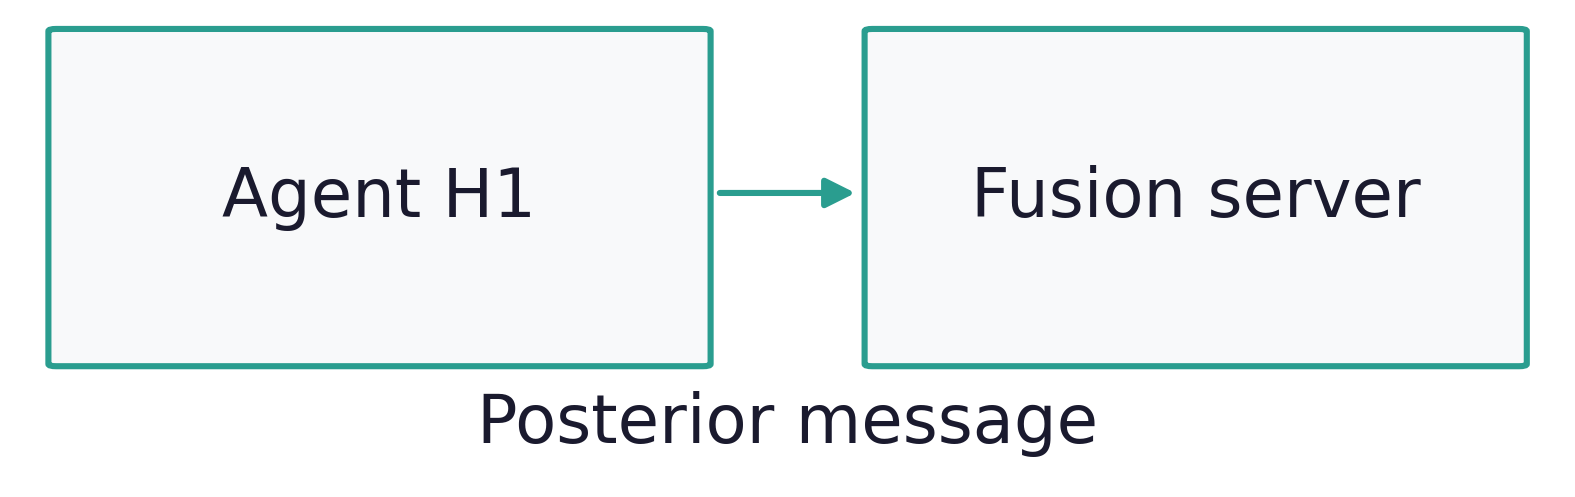
\includegraphics[keepaspectratio,width=0.98\linewidth,height=0.8\textheight,alt={Agent H1 → Fusion server: Posterior message; data\_dependency.}]{../figures/graphical_abstract.slide-network-h1.png}
\refstepcounter{figure}\label{fig:graphical-abstract-slide-panel-32}
\end{figure}
\end{frame}

\begin{frame}{Abstract (part 45)}
\begin{figure}
\centering
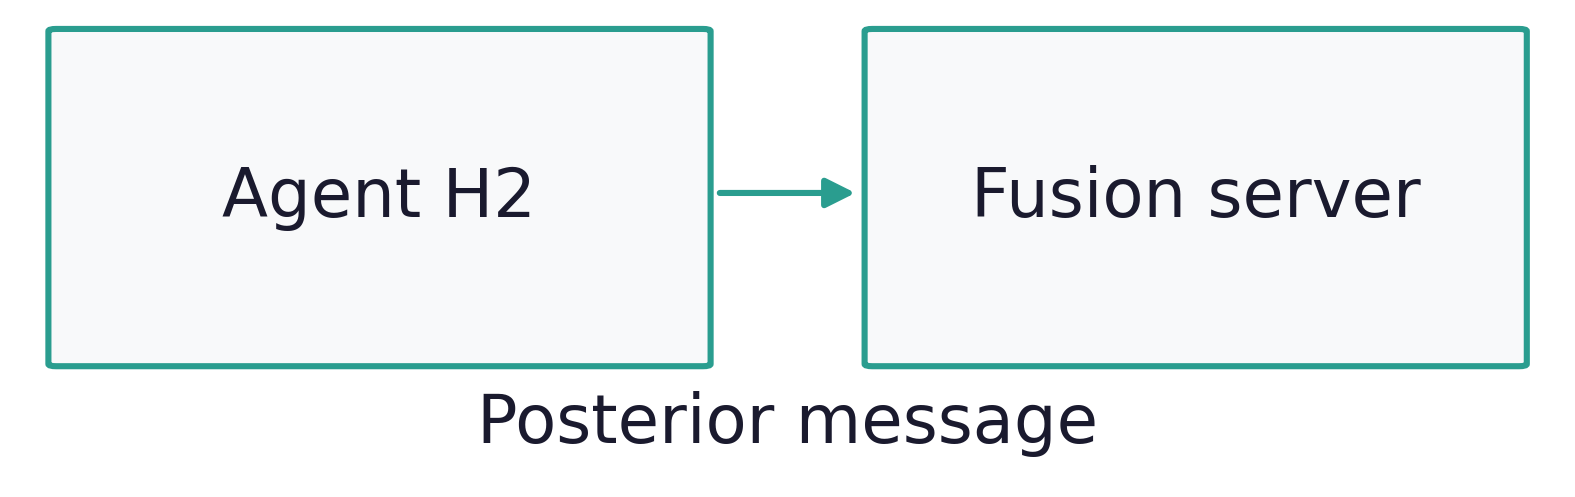
\includegraphics[keepaspectratio,width=0.98\linewidth,height=0.8\textheight,alt={Agent H2 → Fusion server: Posterior message; data\_dependency.}]{../figures/graphical_abstract.slide-network-h2.png}
\refstepcounter{figure}\label{fig:graphical-abstract-slide-panel-33}
\end{figure}
\end{frame}

\begin{frame}{Abstract (part 46)}
\begin{figure}
\centering
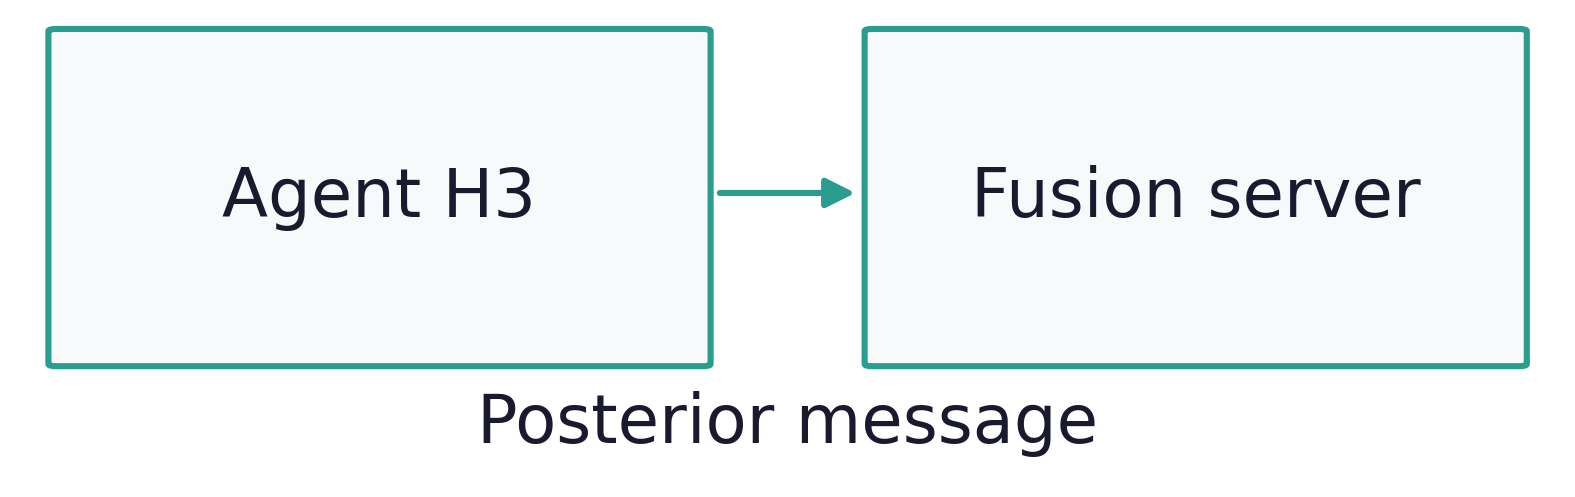
\includegraphics[keepaspectratio,width=0.98\linewidth,height=0.8\textheight,alt={Agent H3 → Fusion server: Posterior message; data\_dependency.}]{../figures/graphical_abstract.slide-network-h3.png}
\refstepcounter{figure}\label{fig:graphical-abstract-slide-panel-34}
\end{figure}
\end{frame}

\begin{frame}{Abstract (part 47)}
\begin{figure}
\centering
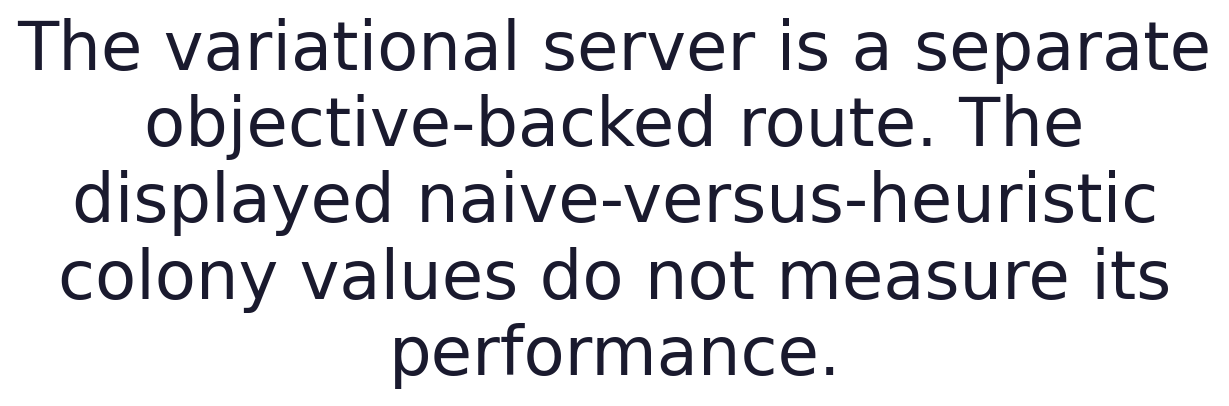
\includegraphics[keepaspectratio,width=0.98\linewidth,height=0.8\textheight,alt={The variational server is a separate objective-backed route. The displayed naive-versus-heuristic colony values do not measure its performance.}]{../figures/graphical_abstract.slide-variational-scope.png}
\refstepcounter{figure}\label{fig:graphical-abstract-slide-panel-35}
\end{figure}
\end{frame}

\end{document}
